\documentclass{article}

\usepackage{setspace}
\usepackage{hyperref}
\usepackage{xargs}                      % Use more than one optional parameter in a new commands
\usepackage[pdftex,dvipsnames]{xcolor}  % Coloured text etc.
\usepackage[colorinlistoftodos,prependcaption,textsize=tiny]{todonotes}
\usepackage{float}
\usepackage{mathptmx}% http://ctan.org/pkg/mathptmx
\usepackage{listings}
% \usepackage[document]{ragged2e} % auto text align left
\usepackage[a4paper, total={6in, 8in}]{geometry}

\title{\textbf{Msc. Thesis} \\
Applied Visible Light Communication for Robotics}
\author{
   Martino Secchi\\
    {msec@itu.dk}\\
    \\
    Supervisor:\\
    Kasper St\o y
}
\date{June 2017}

\begin{document}

\pagenumbering{gobble}
\maketitle
\clearpage

\listoftodos
\clearpage

\tableofcontents
\clearpage
\pagenumbering{arabic}

\abstract{[This is my abstract, what I did and my results, in about 100 words]}

\section{Introduction}
% here, stuff about what the project is about, so the robotics part
% only short digression on vlc, more in the related work section, together with other technologies too
% here goes the robotics stuff, motivation basically, what are the main goals i want to achieve, what will happen in the rest of the thesis


% Intro on vlc
Visible Light Communication, often abbreviated to VLC, is a type of wireless communication achieved with the transmission of signals in the spectrum of visible light.
For most applications, this communication form is implemented through the use of  normal light emitting diodes (LEDs) or fluorescent lamps switched on and off at high rates to produce light signals.
It is gaining increasing popularity as an application of pervasive computing, since many light emitting devices are commonly present in everyday life and used everywhere.
This form of communication has been proven by research to achieve performances comparable to more classic ones, performing well both in speed and distance (section \ref{sectionVLC}).
Although it has some clear limitations, it also provides appealing features in certain contexts.
In general, a VLC system will need a direct line of sight between the source and the receiver, excluding cases where light reflection might be sufficient.
This can be seen as a limitation for obvious reasons, but this characteristic can be exploited to produce interesting features to certain applications.
Communication can in fact be restricted in specific areas delimited by physical boundaries, ideal for localised services or security sensitive applications.
However, communication will result less effective in presence of direct light from other sources, like direct sunlight, and VLC systems are generally designed for indoor usage.
\newline
%situated
A very distinctive trait of VLC systems is that light is a form of \textbf{situated} communication \cite{kasper}, where the message is not necessarily separated from the physical environment in which it has meaning.
This allows to transmit a message that includes additional information embedded in the medium of transmission rather than its content.
In particular, information relative to localisation and direction can just be derived from the light source's position, instead of it being encoded in the message.
This is in general harder to achieve with many other technologies, like WiFi or Bluetooth, that can only give a sense of directionless proximity to the source, at least without employing techniques like triangulation or fingerprinting or sharing a common reference system.
With situated communication, the properties of the transmission can enrich the information to be received, that will be more than just the content of the message.
Very much like human hearing or sight, messages like "I'm here" or "come here" can be fully understood and acted upon when the source of the message can be clearly located.
\newline
%swarm robotics
This characteristic has been proven very useful in the field of mobile robotics, and in particular in \textbf{swarm robotics}.
Mobile robots are by definition able to move in space, and are therefore potentially capable of exploiting the information about direction and relative position of the source of a message.
Swarm robotics is the study and application of a control paradigm used in multi-robot systems, in which usually large amounts of robots interact with each other to form a collective behaviour with the ultimate goal of performing a task.
The strong point of swarm robotics is that relatively simple agents can produce fairly complex swarm behaviours, exploiting constant feedback and communication between the agents.
This research field originates from the observation of emergent behaviour exhibited by social organisms, examples of which can be insects like ants and termites, birds, fish, quadrupeds and bacteria.
This kind of systems rely intrinsically on local communication and mutual localisation between the agents \cite{architecturesswarm}.
A communication method that allows both would therefore allow greater simplicity in the design of such systems.
\newline
Visible light communication has been applied to swarm robotics in numerous occasions, most notably in the Swarm-bots and Swarmanoid projects funded by the European Commission in 2002 and 2006.
In these projects, robotic agents communicate states with RGB LEDs in a colour based system.
Each agent can communicate a state coded into a specific colour, and perceive other agents' states.
This functionality can be used to achieve dynamic shape formation of self assembly robotic agents  \cite{assemblysbots}, or distributed coordination of self organising agents for navigation \cite{distrcoord} \cite{holeavoidance}, navigation and path formation \cite{pathformation}.
\newline
%motivation
These examples, like many others, use a rather reactive approach to obtain and communicate information.
In a colour based system like the before mentioned one, agents simply react to certain colours in predefined ways, like they would do with any other sensory information when the behaviour is programmed.
The same responses could be implemented for other kinds of information, like ones coming from proximity sensors or thermometers, accelerometers, gyroscopes and so on.
There are circumstances however where this kind of reactive approach is not enough, and more complex information need to be passed from one agent to another.
A form of generic communication that still achieves to be local and allows agents to localise each other could contribute greatly to the field of swarm robotics.
Another potential beneficiary could be the field of embodied evolutionary robotics, where agents of a system need to communicate information necessary for reconfiguration of hardware or behaviour, in order to adapt to previously unknown or dynamically changing conditions autonomously \cite{embodiedevolution}.
This kind of complex information could be passed through a generic purpose communication system that allows any kind of message to be sent and received, while still maintaining the advantages of a situated medium of transmission.
%applications
Such a technology could be used in both very simple or more advanced forms, the simplest of which would be mono directional, environment to robot communication.
This could be used in the context of mobile robotics to provide an aid for environment navigation, for example providing useful information about indoor positioning,
or a form of remote control of agents, instructing robots on what actions to perform in predetermined locations, to assist in the execution of specific tasks or location specific services. 
The technology could also be used in a slightly more complex scenario of robot-to-robot 1- or even 2-way communication between multiple agents to enable cooperation, behavioural reconfiguration, hardware/shape reconfiguration, and in general to exchange information.
\newline
%design
The design of a prototype system will help analyse the properties of a generic VLC system, its performances and results in the given applicative scenario of mobile robotics.
The design process will be focused on simplicity and inexpensiveness where possible, by using mostly off-the-shelf and easily obtainable hardware components to achieve sufficient performance within reasonable cost and computational power.
This prototype system will be tested and evaluated both as a general communication system and as a system to be specifically used for mobile robotics.
%requirements
The system will be considered sufficiently performant if it can allow generic messages to be received correctly within a spatial range, and if the source of communication can be localised by the receiver.
The ideal rate of transmission would be any rate that is not noticeable by the human eye and doesn't disturb human observers, while still being registered by specialised sensors.
Research suggests that this rate, known in the field as the critical flicker fusion rate, is close to 65 Hz for spatially uniform light sources, but can reach up to 500 Hz when the light source contains a spatial high frequency edge \cite{eye}.
Normal light emitting diodes will be considered uniform light sources.

\todo{sneak peek in the results?}

\todo{talk about situated communication}

\section{Visible Light Communication}
\label{sectionVLC}
\begin{figure}[hbt]
	\centering
  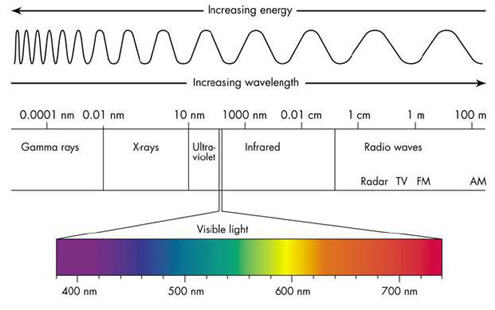
\includegraphics[height=200px]{img/wavelengths}
  \caption{Wavelengths, highlighted visible light band}
  \label{fig:wavelength}
\end{figure}

%intro
Visible Light Communication is a form of optical communication that uses signals in the visible light band to transmit information.
Contrary to the more common fiber-optic communication, VLC is wireless, and transmitted over free space.
In this context, for free space it is meant air, vacuum, or something similar, in contrast to other forms of optical communication that channel transmission into cables or others, like it is for fiber-optic.
Typically, normal fluorescent lamps or LEDs, rather than complex communication devices,  are used to transmit in VLC.
In general, receivers are electronic devices that include one or more photoresistors, in order to measure light signals from a source.
In some cases, digital cameras can also be used to as receivers, but it is a more challenging approach since the frame rate of modern video cameras is generally slow for communication, at around 30 - 60 Hz.
By modulating the light source through a controller it is possible to encode messages from digital form into light signals.
The simplest example of this encoding is a binary representation of data through light, where the presence of light represents a binary 1 and its absence a 0.
This form of communication is a simplified variation of the technology known as Li-Fi, a term that stands for Light-Fidelity.
LiFi and VLC in general can be used in pervasive computing applications, seeing the pervasiveness of light emitting devices everywhere.
Example of devices that could be enhanced with a communication feature are common lamps, both indoor and outdoors, car and traffic lights, commercial signs, even smartphones.
Visible light has been proven by research to achieve good transmission speeds and distances, is user friendly, safe, and easily restrained. 
\newline 
In general, \textbf{LED}s are the preferred light emitters in VLC systems.
The reasons can be several: LEDs can be pulsed at very high speeds without noticeable effect on the lighting and with no damage to the bulb, they last much longer than their competitors and require much less voltage and current.
Compared to halogen, incandescent or fluorescent light bulbs, LEDs do not use tungsten filaments that can get damaged.
Instead, they use a PN junction between two semiconductor materials that, when activated with a suitable voltage, realises energy in form of photons.
Since there is no filament to damage, LEDs can last much longer than other bulbs, and can undergo fast switching without danger.
\todo{maybe have some references here?}
 
 %optical
\subsection{Optical Communication}
Optical communication is allegedly one of the oldest types of communication from a distance in the history of human kind.
Examples of early communication techniques that use light to carry signals can be traced back millennia, with the first lighthouses, navigation lights, beacon fires that would assist in navigation or communicate danger.
It is only with the spread of electricity though, that optical communication technologies could really develop.
Many trace the start of Visible Light Technology back to 1880, when Alexander Graham Bell and Charles Sumner Tainter invented the photophone, a device able to transmit wireless voice messages over several hundred meters modulating sunlight. \todo{reference to photophone}
Since then, optical communication has been developed to include many different variants, the most common of which is \textbf{fiber optic communication}. 
This form of communication sends signals as light pulses through optical fiber.
Optical fiber is a hair-thin, transparent, extremely pure glass or plastic fiber that allows optical signals to travel from one end to the other with very high reliability\cite{opticalfiber}.
The light signal is constantly kept at the centre of the fiber, in its core.
Around the core, there is a layer called cladding, in a material of lower refractive index than the core.
This is to ensure that the light is trapped in the core, exploiting an optical property called total internal reflection.
All around the fiber there is a buffer layer, that protects the fiber itself.
Transmitters are usually LEDs or laser diodes, that can transmit in the visible light spectrum, infrared, or ultra violet.
Infrared light is more common however, because transmission is achieved with less attenuation and dispersion compared to visible light.
Fiber optic communication achieves high bandwidth, long distances, and is not subject to electromagnetic interference, contrary to electrical cabling.
Like fiber optics, also other common optical communication technologies include \textbf{infrared} light (IR) and \textbf{ultraviolet} (UV).
Infrared communication is used over free space to achieve short and long range communication.
As an example, most remote controllers use infrared signals, often modulated to to prevent interference form other light sources.
 
%indoor
\subsection{Indoor positioning}
In 2015, Philips released their LED based indoor positioning system as part of a collaboration with the supermarket chain Carrefour\cite{philps}.
The first installation has been delivered in one of their supermarkets in Lille, France.
Similar installations have been done for other retailers in D\"usselforf (Germany), Dubai (Emirates), and Eindhoven (Netherlands).
LED fixtures inside the shop transmit unique VLC signals that are received by smartphones through their front camera.
Paired with a cloud based database, the light signals are translated into a specific indoor position inside the shop, to help the user determine his/hers location.
To every product and offer in the shop is also associated a specific position inside the shop, conveniently displayed on a map for helping navigation and path finding. 
The system achieves illumination of the shop, energy saving for the lightning, and an indoor positioning system.
The system is intended for large retailers to assist shoppers find products and promotions faster, and navigate through the aisles, but can potentially be used in a wider range of applications.
For example it could be used in hospitals and elderly care facilities to track resources and people \cite{arduinobasedindoors}, or to assist/control indoor robotic vehicles in large warehouses.

%ronja
\subsection{RONJA}
RONJA (Reasonable Optical Near Joint Access) is a visible light communication system that operates wirelessly in free space using light beams that can achieve 10 Mbit/s full duplex Ethernet point-to-point link at 1.4 km of distance \cite{ronja}.
The entire system is labeled as User Controlled Technology: blueprints, schematic, building instructions and software components are all open source and freely available, the design is published under the GNU Free Documentation License.
It is a project originated in the Czech Republic and released in 2001 by Twibright Labs.
The group provides the instructions and the design of the system, leaving the purchase of the components and the assembly of the system to the end user.
In 2010 it has been estimated that up to 2000 links have been built worldwide \cite{ronjaestimation}.
Of the three official model designs, only two use visible light (red), while the third uses infrared.

%lifi
\subsection{Li-Fi}
The term Li-Fi was first introduced by a german physicist, Harald Haas, co-founder of PureLiFi, in occasion of a TED Global talk on Visible Light Communication in 2011 \cite{tedtalk}.
Since then, the term has been reported in many articles and has gained popularity as a common synonymous for Visible Light Communication.
After the name was adopted by the Optical Wireless Communication (OWC) community with the launch of the LiFi Consortium in 2011, an industry group that promotes OWC technologies, it can be sometimes extended to describe general wireless data access points that use light, visible or otherwise.
This includes also the infra-red and ultraviolet band.\\
The main reason why this technology is quickly gaining popularity in the research is because it potentially allows to unlock a vast amount of electromagnetic spectrum in the visible light region, unused for transmission.\cite{haas1}
This has been seen as a promising reaction to the saturation of the Radio Frequency (RF) spectrum, a very likely outcome of the huge success of wireless technology, also predicted by the US Federal Communication Commission\cite{crisis}. 
A second reason is that transmission through light can achieve surprising high speeds.
Starting from 2010, research had been able to improve the transmission rate further and further.
In his TED talk in 2011 Haas demonstrated real time video streaming from a white LED at data rates up to 130 Mbps\cite{tedtalk}, while another group achieved over 513 Mbps\cite{500Mbps}.
In the following years, there have been continuous reports of improved data rates in transmission.
A single white LED has been proven to transmit from about 1 Gbps\cite{1Gbps}, up to 3.5 Gbps\cite{3.5Gbps}, while 3.4 Gbps have been demonstrated with a single RGB LED\cite{3.4Gbps}.\\
This rates can be further improved by the use of arrays of light sources and more complex systems.
The Mexican software company Sisoft together with scientists from the Autonomous Technological
Institute of Mexico in 2014 reached the surprising data rate of 10 Gbps, setting the record.\\
Other appealing aspects to this technology are the low cost of implementation for the use of off-the-shelf LED bulbs and its security, for the reason that communication can be eavesdropped only in direct line of sight within short distance.\\
There are a few groups that are leading the research in the field of Visible Light Communication.
One of these is the Li-Fi R\&D Centre at the University of Edinburgh, of which prof. Harald Haas is the director.
Another very important research group operating in the same area is Disney Research, often in collaboration with ETH Zurich.
Another group worth mentioning is the Li-Fi Consortium, an international organisation formed by companies in optical wireless communication technology and research institutes.
A good part of the research is also carried out by multiple other research groups worldwide, especially in Asia and India in particular.

%standards
\subsection{Standard and specifications}
\label{modulschemes}
Visible light communication is regulated by a standard similar to the one of wireless networks, in the same IEEE 802 family.\cite{IEEE}
The IEEE 802.15.7 standard defines a draft of the physical layer (PHY) and the media access control (MAC) layer for VLC. 
According to Gordon Povey, former CEO at PureLiFi\cite{poveyspec}, the MAC layer as of April 2011 supports three multiple access topologies: peer-to-peer, star configuration and broadcast mode.\\
The Physical layer is divided into three types, that use different modulation schemes.
The three modulation schemes are: 
\begin{itemize}
\item On-Off Keying
\item Variable pulse position modulation (VPPM)
\item Colour shift keying (CSK)
\end{itemize}
\textbf{On-Off Keying}\newline
On-Off Keying is the simplest modulation scheme. 
In this scheme, a digital 1 is represented by the light state being on, and 0 otherwise.
In the 802.15.7 standard, Manchester coding is used to ensure the period of each pulse is the same.
This type of encoding, instead of having a digital 0 represented by a low signal and a digital 1 by a high signal, encodes each data bit as either low then high (1), or high then low (0), in equal time.\\
\newline
\begin{figure}[H]
\centering
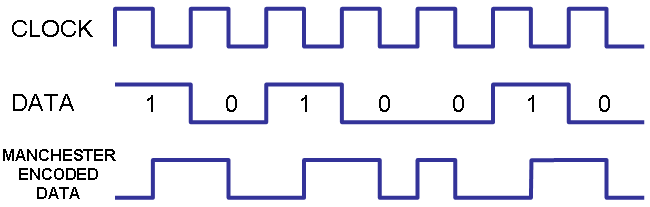
\includegraphics[scale=0.3]{img/ookmodulation}
\caption{OOK modulation using Manchester coding.}
\label{fig:ookmod}
\end{figure}
\textbf{Variable pulse position modulation (VPPM)}\newline
VPPM is similar to pulse position modulation (PPM), in which the data is encoded using the position of the pulse within a set time period.
In this modulation scheme, light dimming is allowed as long as the period containing the pulse is long enough to allow different positions to be identified. 
As in the Manchester coding a positive pulse at the beginning of the period followed by a negative pulse at the end can represent a digital 0, and a 1 is represented by a negative pulse at the beginning followed by a positive one at the end.\\
\newline
\begin{figure}[H]
\centering
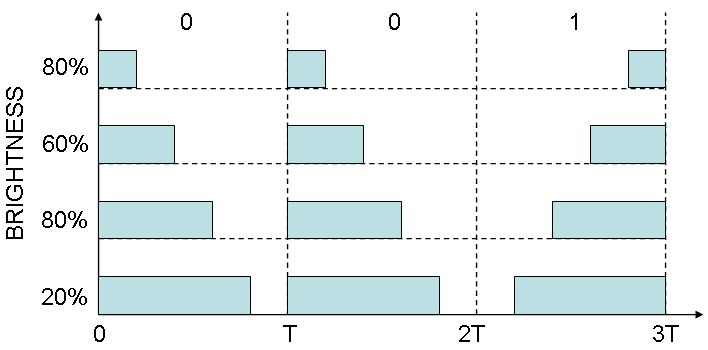
\includegraphics[scale=0.3]{img/VPPM}
\caption{Variable pulse position modulation to support light dimming.}
\label{fig:ookmod}
\end{figure}
\textbf{Colour shift keying (CSK)}\newline
This scheme allows the light intensity to be constant by encoding the information in the colour of the light.
For implementing this kind of transmission the system must use RGB type LEDs.

%other technologies
\subsection{Comparison with other technologies}
In this section, a comparison between common wireless technologies in relation to VLC is presented.
The data is partially based on the article "Comparative Performance Analysis of Wireless
Communication Protocols for Intelligent Sensors
and Their Applications" (2014) \cite{comparison}.\\
\newline
  \begin{tabular}{l| c c c c}
    Technology & frequency band & range & max. data rate & source localisation\\
    \hline
   WiFi & 2.4 GHz / 5 GHz & 10-100 m &  54 Mbps & no\\
   Bluetooth & 2.4 GHz & 10-100 m & 1-3 Mbps & no \\
   UWB & 3.1 - 10.6 GHz & 10-100 m & 110 Mbps & no\\
   ZigBee & 0.8 - 2.4 GHz & 10-1000 m &  250 Kbps & no\\
   Mobile broadband 3G & 0.85/ 0.9/ 2.1 GHz & 2-35 km &  2-21.6 Mbps & no\\
   Infrared & 430 THz to 300 GHz & 0.1 - 1 m to 1.25 km & 1 Gbps & yes \\
   Visible light & 430-770 THz & 0.1 m to 2 km & 10 Gbps & yes \\
  \end{tabular}













\section{System Overview}
%[In the next chapters I describe the overall characteristics and limitations that a VLC system should present according to my findings, identify the variables involved and the set of parameters necessary for it to work. This chapter should provide a useful starting point for whoever plans to implement one in practice What does one need to make his own VLC system?]
%Structure of a VLC system: logical layer, control layer, physical layer. Analysis and characteristics of the three.
%logical abstraction
Every visible light communication system shares the same underlying structure, as also general other communication systems.
Communication needs to be established between two ends, one end that acts as a transmitter and the other that acts as a receiver.
There are at least three levels of abstraction needed to transform a digital information into a signal that can be sent and received, and these can be defined as: 
\begin{itemize}
\item \textbf{logical layer}, where the information is handled at a software level
\item \textbf{control layer}, responsible of managing the variations of the physical property used for communication in a organised and structured manner
\item \textbf{physical layer}, where the properties of the communication are limited by the physical properties of the signal and the characteristics of the hardware
\end{itemize}
Each of these levels present different characteristics that combined form the overall performance of the system.\\

%physical
In VLC, the transmitter end of the communication operates on a light emitter to vary a property of the light depending on the modulation scheme used (see \ref{modulschemes}), like brightness or colour.
The receiver on the other end needs to be able to detect such variations in a measurable manner.
This level can be described as the \textbf{physical layer} of the communication.
At this level, the system's performance can be influenced by physical properties of the hardware, like maximum brightness of the light emitter, warmup time or time that the emitter takes to turn on, but also by other factors, like distance between the two ends, the medium of transmission, the angle of incidence of the light between transmitter and receiver and so on.\\

%control
This variations in the properties of light need to be controlled and organised to carry specific information.
A \textbf{control layer} is necessary in order to make the link between logical information and variation of physical property.
This layer is of critical importance for the performance of any system, since it influences the frequency of the physical variations which results in the rates for transmission and reception.
Factors that are to be considered in this layer are directly linked to the hardware components, namely any characteristic that influences the overall speed of transmission/reception, like clock rates of the micro controllers, speed of the transistors used and so on.\\

%logical
The outer most level of abstraction is the \textbf{logical layer}, where information is handled and manipulated at a software level.
For a transmitter, this layer produces the instructions to pass on to the control layer in order to generate a signal given a specific information. 
This process can be seen as the logical encoding of the information, ready to be transferred and become physical encoding.
At the opposite end of the transmission, the logical layer of a receiver is given data about physical variations measured by the sensor(s) used in the system, and needs to reconstruct and interpret such data back to the original information.
Contrary to the previous layers, the performance of the logical layer doesn't rely much on the hardware and the physical characteristics of the components, but rather on the software techniques and algorithms that implement it.
A well structured logical layer could potentially add more reliability to an otherwise uncertain medium of communication, allowing a stricter control on the traffic and implementing recovery options in case of mistakes.

\begin{figure}[hbt]
  \centering
  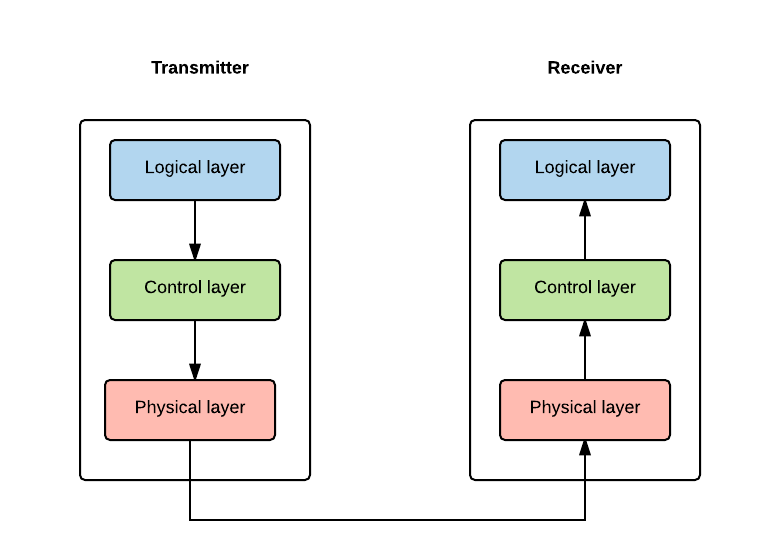
\includegraphics[height=180px]{img/LCP}
  \caption{Conceptual layers of the system.}
  \label{fig:lcp}
\end{figure}


%prototype architecture
\subsection{Experimental setup}
\label{expsetup}
In order to verify feasibility, investigate characteristics and test performance of general VLC systems, a prototype system has been developed.
The system is composed of two main modules: a transmitter module, and a receiver.
The transmitter module uses On Off Keying with Manchester Coding (see \ref{modulschemes})  to convey signals with light.
In order to allow testing, this module takes some arbitrary input from a user, encapsulates the information and encodes it to produce variations in light intensity, through the control of a light emitter.
The receiver side measures the light variations through the use of a photoresistor, or light sensor, reconstructing and interpreting the sensor data back into the original messages. 
If the message that is received matches the one that is sent, the communication is considered successful.
Each module includes different components, listed in section \ref{components}.
Fig. \ref{fig:sys over} shows an overview of the prototype's architecture.

\begin{figure}
\centering
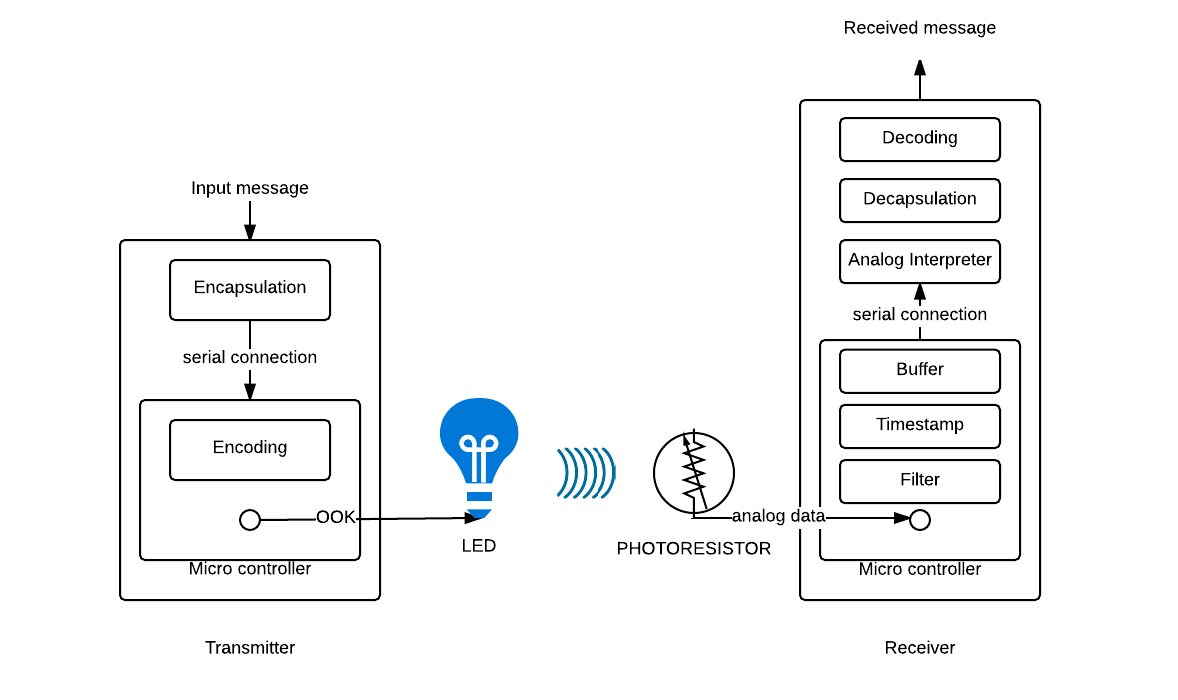
\includegraphics[height=200px]{img/sysover}
\caption{Prototype system.}
\label{fig:sys over}
\end{figure}

%transmitter
\subsubsection{Transmitter}
Transmission starts from a terminal, where a user can input messages as strings. These are then encapsulated into Protocol Data Units (PDUs) and sent to a micro controller through a serial connection.
In this case, the micro controller that was used for transmission is an Arduino board.
The board encodes the received bytes into Manchester Code, and then controls the light signal by switching on and off the emitter accordingly.
A light emitting diode is the furthest end of the transmitter module.
For this part, multiple setups have been tried.
The fastest emitter that has been tested is single low power LED connected to the board and powered directly by it, which allows very fast switching.
LEDs are preferable compared to incandescent or fluorescent light bulbs, since they are generally faster and are not damaged by the switching like the other options.
All other kinds of bulbs, halogen, incandescent and fluorescent, have tungsten filaments that get damaged by the thermal shock of the switching, so they require more time, more power and do not last as long if compared to LEDs.
A second setup has also been tested with a commercial LED bulb powered by an external power source (mains electricity), and controlled by the board through a switcher. 
A bigger bulb, powered by a bigger power source, can achieve higher luminous intensities and reach longer distances.
However controlling external power sources is lightly more complex, and especially so with alternating current.
This second setup with the LED light bulb was not used in the final stages to achieve communication, for various limitations encountered in the process.
Most of the results achieved later on will be referring to the first setup with the fast switching low power LED, unless otherwise specified.


%\todo{in the experimental setup, it's considered almost exclusively low power DC LED, discuss role of big bulb}

%receiver
\subsubsection{Receiver}
%Sending light signals is not too complicated, what really is the core of the project is to read such signals and interpret the sensor data correctly.
The signal is received by a photodiode read as analog input by a micro controller.
On the board, values are software-filtered to reduce noise, and sent to the receiving terminal with a timestamp.
The board and the terminal are connected through a serial connection.
Some controllers could read directly analog input and perform the remaining processes to interpret the signal, with enough computational power.\\ 
For this application, the final terminal is a Raspberry Pi, since it has a good power/size ratio for the designed purpose and allows a simple prototyping process. The micro controller in between the sensor and the terminal is necessary to read and forward analog data, which is not possible directly from the Raspberry Pi.\\
On the final terminal, the variations of sensory data are interpreted as sequences of digital 0s and 1s, finally decapsulated and decoded back into a message.

%components
\subsection{List of components}
\label{components}
Each module of the prototype system is composed of different components, listed in the following.\\
Transmitter:
\begin{enumerate}
\item personal computer as main terminal for user input and information processing
\item Genuino Uno micro controller board, based on ATmega328P \cite{genuinouno}
\item Light emitting diodes:
\begin{enumerate}
\item low power LED, Blue 10 mm, forward voltage 3.0-3.4VDC, luminosity of 8 000-10 000 MCD, directional, 30$^{\circ}$ viewing angle \cite{ledDS}
\item commercial LED bulb, 230 V AC, 3 W, 240 lumen, directional, 120$^{\circ}$ viewing angle 
\end{enumerate}
\item Solid State Relay for Arduino, 5V activation, 240V load
\end{enumerate}
Receiver:
\begin{enumerate}
\item Photoconductive Cell VT900
\item Genuino Yun micro controller board, based on ATmega32u4 \cite{arduinoyun}
\item Terminals:
\begin{enumerate}
\item personal computer for test of communication
\item Raspberry Pi 3 Model B to be applied on a mobile robot \cite{raspberrypi}
\end{enumerate}
\end{enumerate}

\subsection{Wiring}
In figure \ref{fig:wiringDC} is shown the wiring of all the components of the prototype system.

\begin{figure}[hbt]
\centering
  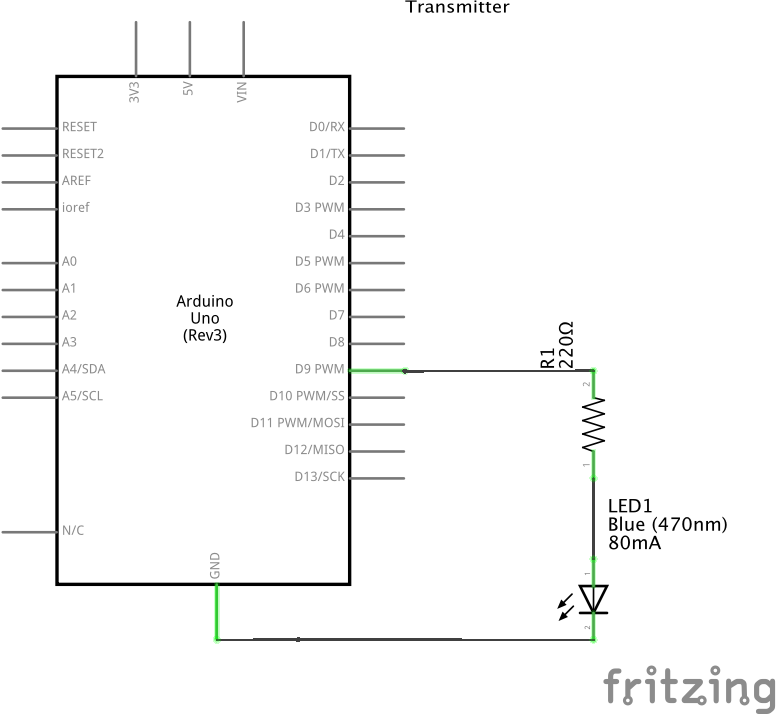
\includegraphics[height=150px]{img/transmitter_schem1}
  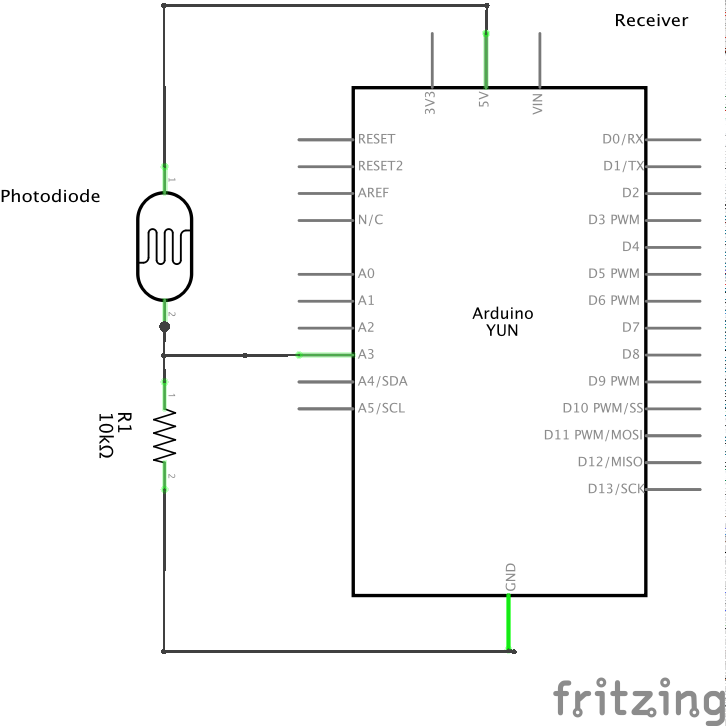
\includegraphics[height=150px]{img/receiver_schem1}
  \caption{Wiring of the boards and sensors.}
  \label{fig:wiringDC}
\end{figure}





% I think sections 3.1 to 3.3. will probably become chapters. In each of them you have to describe the motivation, requirements, choices made, experimental setup, experiments, result in the light of the requirements. Hence, they can become quite big... 

\section{Physical layer}
\label{physical}

\todo{what requirements do I need to meet here?}

This layer is about physical properties of the hardware and the signal itself.\\
In this section these properties will be analysed through the aid of various experiments performed on the prototype system.
%motivation
This is a first step in understanding the potential and the limitations of a system, because whatever limitation derives from the physical layer, it will be a hard limitation that will affect the entire system.
Therefore, starting to look at physical constraints of the system will give a good overview of what can be achieved and what cannot early on, before the rest of the designing process.
% experimental setup
All the following experiments will be performed on the prototype system as described in section \ref{expsetup}, with the use of the low power 10mm LED unless otherwise stated.
%why brigthness in %
A remark on the experiments that will follow is that brightness will be always reported in percentage.
This serves the purpose of making the data applicable in general cases, even with different light sources.
The LED used for testing produces a luminous intensity of about 8 000 to 10 000 MCD at 25$^{\circ}$ \cite{ledDS}.

%warmup
\subsection{Warmup time}

%These are stats for warmup only at dark
\begin{figure}[h]
\centering
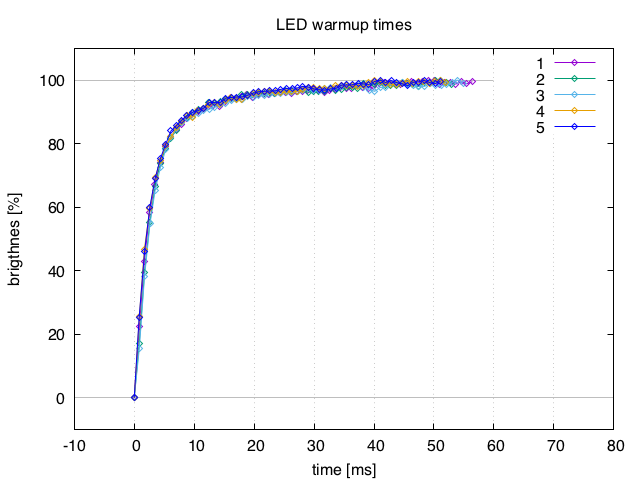
\includegraphics[height=140px]{img/warmup1}
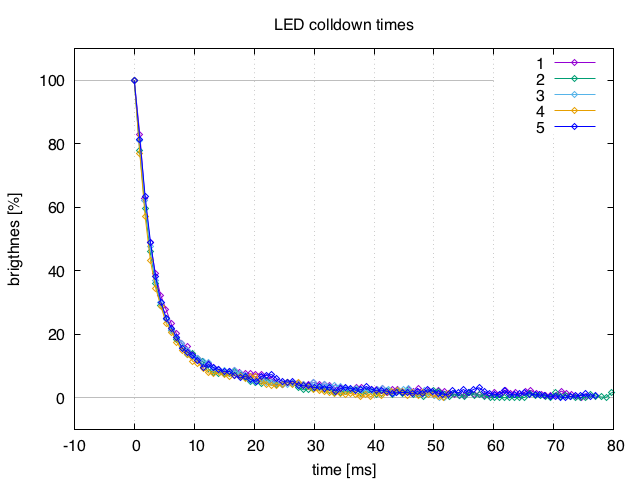
\includegraphics[height=140px]{img/warmdown1}
\caption{LED warmup and cooldown times.}
\label{fig:warmup}
\end{figure}

The speed of light transmission depends in primis on the speed at which the light itself can be turned on and off.
Figure \ref{fig:warmup} shows the warmup times for the low power LED over multiple instances, meaning the time that it takes for turning the light completely on from completely off, and vice versa.
These measurements depend on the reception rate of the system, which will be discussed in section \ref{recrates}.
Table \ref{tab:warmup} shows the times for the LED to switch between specific brightness levels.
Each row represents the time to reach the level on each column, for example the first row represents the time to reach any brightness level starting from 0\% brightness.
The table works both ways, meaning it shows the time for the warmup as well as the time for the cool down of the LED.
As another example, the last row shows how long it takes to reach any level from a completely ON state, meaning starting from 100\% of brightness.

\begin{table}[hbt]
\centering
  \begin{tabular}{ l | c c c c c c c c c c c}
    & 0\% & 10\% & 20\% & 30\% & 40\% & 50\% & 60\% & 70\% & 80\% & 90\% & 100\% \\
    \hline
0\% & - & 0.3 & 0.66 & 1.08 & 1.52 & 2.12 & 2.82 & 3.78 & 5.38 & 10.4 & 50.66 \\
10\% & 55.88 & - & 0.36 & 0.78 & 1.22 & 1.82 & 2.52 & 3.48 & 5.08 & 10.1 & 50.36 \\
20\% & 61.86 & 5.98 & - & 0.42 & 0.86 & 1.46 & 2.16 & 3.12 & 4.72 & 9.74 & 50.0 \\
30\% & 63.76 & 7.88 & 1.9 & - & 0.44 & 1.04 & 1.74 & 2.7 & 4.3 & 9.32 & 49.58 \\
40\% & 64.9 & 9.02 & 3.04 & 1.14 & - & 0.6 & 1.3 & 2.26 & 3.86 & 8.88 & 49.14 \\
50\% & 65.76 & 9.88 & 3.9 & 2.0 & 0.86 & - & 0.7 & 1.66 & 3.26 & 8.28 & 48.54 \\
60\% & 66.4 & 10.52 & 4.54 & 2.64 & 1.5 & 0.64 & - & 0.96 & 2.56 & 7.58 & 47.84 \\
70\% & 66.98 & 11.1 & 5.12 & 3.22 & 2.08 & 1.22 & 0.58 & - & 1.6 & 6.62 & 46.88 \\
80\% & 67.48 & 11.6 & 5.62 & 3.72 & 2.58 & 1.72 & 1.08 & 0.5 & - & 5.02 & 45.28 \\
90\% & 67.92 & 12.04 & 6.06 & 4.16 & 3.02 & 2.16 & 1.52 & 0.94 & 0.44 & - & 40.26 \\
100\% & 68.28 & 12.4 & 6.42 & 4.52 & 3.38 & 2.52 & 1.88 & 1.3 & 0.8 & 0.36 & - \\
  \end{tabular}
  \centering
  \caption{Warmup times in [ms] of the LED, for specific levels of brightness. Row: from brightness, Column: to brightness.}
  \label{tab:warmup}
\end{table}

From the table as well as from fig. \ref{fig:warmup}, it can be seen that the LED is slightly faster at being turned on rather than off.
Also pretty indicative is the fact that about 90\% of the time used for turning a LED completely on or completely off, is spent to make a variation in the last 20\% of brightness levels, which means that a LED can reach a reasonably high brightness in a time relatively small compared to its full potential.
Interesting for later sections is that 50\% of the brightness can be reached in about 2 ms.

%distance
\subsection{Distance}
\label{distancephy}
Another factor that might affect the communication over light is the distance between emitter and sensor, closely bound with the brightness reachable from the light emitter and the presence and weight of light interference.
Intuitively, brighter lights will be visible from farther.
A low power LED cannot reach high levels of brightness, therefore it won't be visible at long distances.
Table \ref{tab:distancesphy} shows the results of different measurements taken at increasing distances sensor to light source.
Two different light sources has been tested, the low power (5V) LED and a commercial LED bulb powered by mains electricity (240V).
The reference for maximum brightness is achieved with a distance of 0 cm between receiver and light source, with the two nearly touching, represented as a 100\% of brightness.
Figure \ref{fig:distancephy} shows the measurements of the same experiments in a graphical manner, only for the low power LED.
In the figure, each colour represents a different distance, and each peak a different experiment.
The experiment was performed in a dark environment, minimising interference from other light sources.

\begin{table}[hbt]
\centering
  \begin{tabular}{c | c || c}
    distance & max. brightness LED & max. brightness bulb \\
    \hline
    0 cm & 100\% & 100\% \\
    10 cm & 42.81\% & 73.31\%\\
    20 cm & 14.28\% & 53.59\%\\
    30 cm & 8.57\% & 40.60\%\\
    40 cm & 5.00\% &31.55\%\\
    50 cm & 3.57\% & 25.03\%\\
    100 cm & 2.14\% & 10.27\%\\
    200 cm & - & 3.81\% \\
  \end{tabular}
 \caption{Maximum brightness over different distances.}
  \label{tab:distancesphy}
\end{table}

\begin{figure}[hbt]
	\centering
      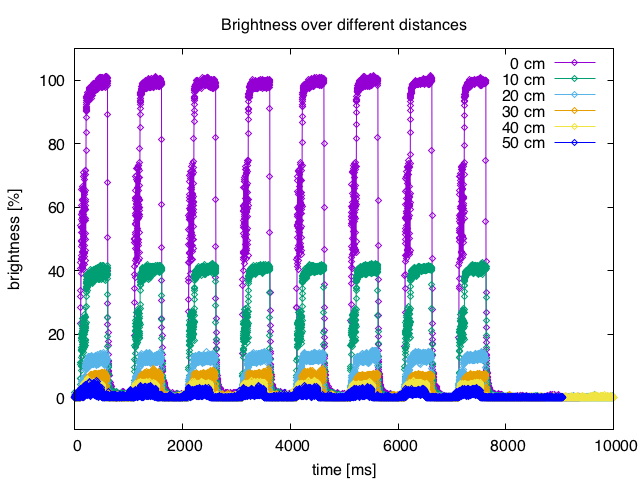
\includegraphics[height=180px]{img/distancephy}
  \caption{Brightness at different distances, low power LED.}
  \label{fig:distancephy}
\end{figure}

From the table and figure it can be seen that the maximum brightness registered from the sensor drops decidedly with increasing distance.
This obviously makes reliable communication over long distances harder.
The comparison between the two light sources clarifies the role of brightness in achieving certain distances.
The LED bulb has registered a brightness 5 to 6 times more intense than the low power LED, and clearly is able to reach longer distances.
The bulb has a wider viewing angle of $120^{\circ}$, compared to the $30^{\circ}$ of the low power LED, and can seemingly reach about 4 times more transmission range.\\
Another important implication with this results is the role of noise in the reception.
Noise doesn't scale with the communication, meaning that if the maximum brightness perceived at a certain distance is 50\% of the brightness at 0 distance, the noise in this first case is not 50\% of the one used for reference, but stays constant.
This means that the lower the variation perceived, the more noise will play a role in the communication.
A remark on the experiments performed is that both lights used for testing are directional, with an optimal viewing angle of about 30$^{\circ}$ from the centre of the emitter for the LED and 120$^{\circ}$ for the bulb. 
The receiver, at the different distances, was always placed in the optimal viewing point in relation to the light emitter direction.


%ambient
\subsection{Interference from ambient light}
Previous data about times to reach maximum brightness were measured in a condition of full darkness of the environment surrounding the light source, at minimal distance between transmitter and receiver.
But visible light communication is not necessarily used with this restriction, it is in fact meant to be used over an open space, wirelessly,  meaning that interference from natural light or other light sources is very likely.
 Experiments have been performed to quantify the influence of ambient light on potential transmission.
 This is done by comparing the difference between the brightness measured by the sensor when the transmitter is turned on and the one when the transmitter is turned off.
 This represents the maximum potential amplitude of a signal.
 This difference will be measured without ambient light interference and used as a reference for the measurements that occur with ambient light interference.
 Since communication  will later rely on the quantification of light variations, it's important to establish if this variations will be substantially different with or without interference present.
 For these experiments, for ambient light it is meant light from any source that is not directed to the receiver but naturally permeates the environment surrounding the system.
 If the variation ON/OFF in a fully dark environment is represented as 100\%, the experiment shows that this difference is between 100\% and 120\% when ambient light is present, averaging at around 110\%. 
Measurements were taken at 0 distance and with direct exposure.
This increase could be explained with a higher sensibility of the sensor when exposed to higher levels of base brightness.
This suggests that ambient light interference doesn't affect transmission quality, at least in optimal conditions, with limited ambient light with no direct source pointing at the sensor and without accounting for distance.
Introducing distance as a parameter though, it appears that light intensity decreases faster over distance when in presence of other light sources.
Table \ref{tab:distancesphyINT} shows the results of testing the maximum brightness received over different distances, with presence of natural light.
The source of the ambient light does not face the sensor directly for these measurements.
The table also compare the results of the same tests performed in a completely dark environment.
Figure \ref{fig:distanchephyINT} shows the same results graphically.

\begin{table}[hbt]
\centering
  \begin{tabular}{c c l}
    distance & max. brightness, dark & max. brightness with natural light \\
    \hline
    0 cm & 100\% & 100\%\\
    10 cm & 42.81\% & 26.28\%\\
    20 cm & 14.28\% & 12.16\%\\
    30 cm & 8.57\% & 7.44\%\\
    40 cm & 5.00\% & 4.78\\
    50 cm & 3.57\% & 4.21\%\\
  \end{tabular}
 \caption{Maximum brightness over different distances, with interference from natural light.}
  \label{tab:distancesphyINT}
\end{table}

\begin{figure}[hbt]
\centering
  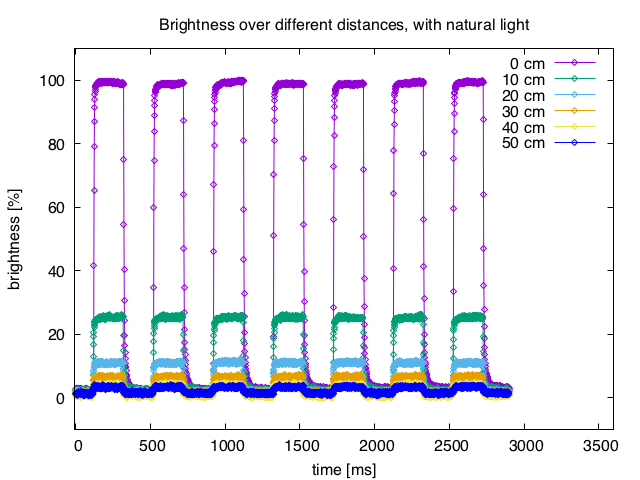
\includegraphics[height=180px]{img/distancephyINT}
  \caption{Brightness at different distances, low power LED with natural light interference.}
  \label{fig:distanchephyINT}
\end{figure}


%angle
\subsection{Angle}
In addition to the previous factors, also alignment between the light emitter and the light sensor might be of relevance when establishing communication between the two ends, under certain circumstances.
So far, in all of the communication tests performed on the system, the receiver was always in direct line of sight with the light emitter and centred to its focus.
However,  if the light source is directional or semi-directional, the angle of incidence would affect the ability of the sensor to register light variations.
This could also be the case for omni-directional light sources, when reflection of the light would be critical for it to reach the sensor.
For example, the light source could not be bright enough to reach reflecting surfaces or these could be absent.
In the case of a regular room as the location of the communication system,  the light source must be powerful enough to either reach the sensor directly with sufficient intensity, or to reach it indirectly by reflecting on the walls, ceilings or other surfaces.
Experiments have been performed with different angles to show how this factor affects overall reception with a directional light source.
The measurements have been taken at a distance of 10 cm between light source and sensor, in a otherwise dark environment.
\begin{table}[hbt]
\centering
  \begin{tabular}{c c}
    Angle & max.brightness \\
    \hline
    0$^{\circ}$ & 100\% \\
    40$^{\circ}$ & 60\% \\
    60$^{\circ}$ & 50\% 
  \end{tabular}
  \caption{Maximum brightness measured at different angles.}
  \label{tab:anglesphy}
\end{table}
These results suggest that the larger the angle of exposure, the less powerful the reception. 

\begin{figure}[hbt]
\centering
  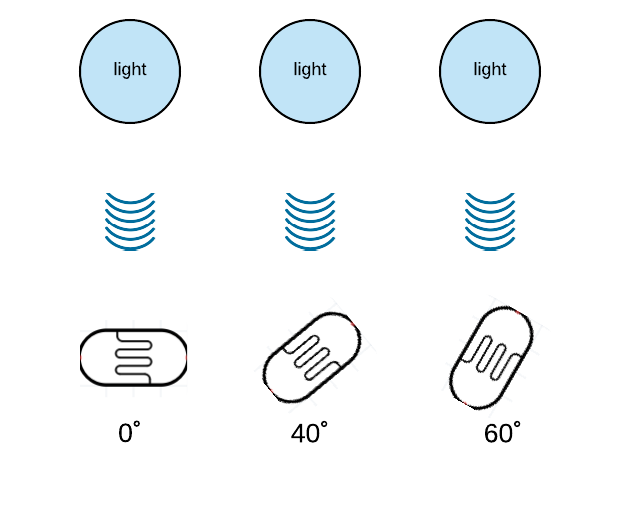
\includegraphics[height=140px]{img/angles}
  \caption{Sensor receiving light from the transmitter at different angles.}
  \label{fig:angles}
\end{figure}


%power ac vs dc
\subsection{Powerful lights and power source}
\label{acphy}
As can be deducted from the previous results, brighter and faster light sources are preferred to achieve better communication, preferably with an alignment between receiver and transmitter and no interference.
These are the optimal conditions for visible light communication. 
Sources that can turn on and off faster can potentially allow faster switching, which in turn allows faster communication.
Light sources that are brighter can be perceived at longer distances, and are less subject to interference.
Such lights have a higher power consumption than less performant ones.
If the vision is to have a smart environment with lights that serve the double purpose of lighting the environment for humans and transmit information to devices, the most natural thing would be to connect these lights to mains electricity like any other lamp.
This power source potentially allows the usage of much more powerful light bulbs then the low power LED used in the prototype.
In Europe, electric power supply for mains is of 230 V at a frequency of 50 Hz \todo{reference mains information.}.
A distinctive trait of this power source is that it uses Alternating Current (AC).
Alternating current periodically reverses direction whereas direct current (DC) always flows in the same direction.
AC voltage can be expressed by a sinusoidal function, which means the current will vary its intensity in time.
Current will be higher near the peak, and lower near the time of the periodic switch in direction. 
This behaviour is clearly represented in figure \ref{fig:warmupAC}, when the light is ON after the warmup in the figure on the left, or before the cool down in the figure on the right.
The ON/OFF difference when measuring the light intensity with the receiver is over 500\% bigger than the LED of the prototype system, with similar rise speeds.
However, the fluctuations of AC during the ON state make it harder to use it for communication using On Off Keying, since that modulation scheme relies on variations in intensity.
A way around this would be to convert AC to DC with a process called rectification \todo{reference rectification}.
This involves the use of a capacitor connected between AC V$^{+}$ and Ground,  which lowers the amplitude of the AC significantly thus producing something very similar to DC.
Another problem to face however, as shown in the picture, is that these LED bulbs have a much slower fall time when switched off, which also would affect the switching frequency during transmission.

\begin{figure}[h]
\centering
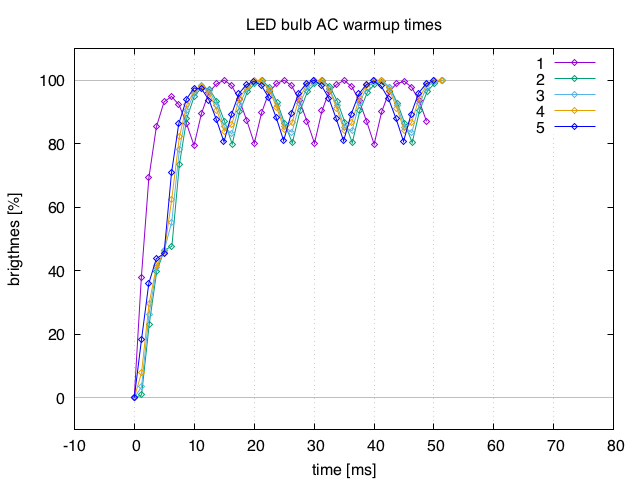
\includegraphics[height=140px]{img/warmup2}
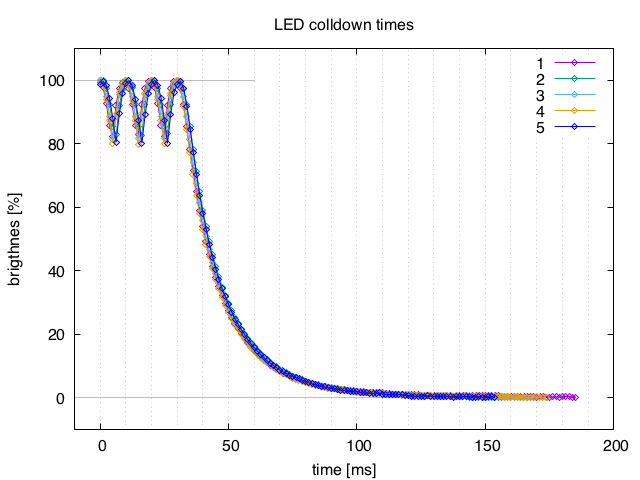
\includegraphics[height=140px]{img/warmdown2}
\caption{AC bulb warmup time, and phases of alternating current.}
\label{fig:warmupAC}
\end{figure}


\section{Control layer}

\todo{what requirements?}

%layer overview
This layer is responsible of connecting the physical and the logical layers of the system, connecting the physical variations that produce the signal with the logical information they carry.
For a transmitter this translates to the process of producing variations of the physical properties in a structured way according to what dictated by the logical layer, in a way that these variations reflect the information given.
For the receiver, the control layer is responsible of reading the values from the sensory layer and forward them to the logical layer, perform filtering and other minor operations.
In the prototyped system, this layer is physically represented by micro controller boards connected with a terminal through a serial connection on one side, and with the components of the physical layer on the other.
This layer is crucial for establishing performance of the system in terms of \textbf{rates}, as in how many values can be read from a sensor per time unit for reception, and how fast can a signal be sent to control the light emitter for transmission.

%serial connection
\subsection{Connection to the logical layer}
Being in the middle of the system, this layer has two connections, one outgoing and one incoming.
The transmitter will have an incoming connection with the logical layer and one outgoing to the physical, while the receiver will have an outgoing connection to the logical layer and one incoming from the physical layer.
Since this layer is the one that produces transmission and reception rates, it's worthwhile to spend some time in analysing both types of connections, because the sum of both will result in the overall performance of this layer.
Transmission rate, as will be discussed, depends on the speed of the outgoing connection from control layer to the physical layer for obvious reasons.
However, the speed of the incoming connection from the logical layer would also play a role.
The same discussion applies for the reception rates, in reverse.
In the prototype, the connections between control and logical layer are implemented as serial connections between the controller board and the terminal where the logical layer is running.
Both boards are Arduinos, and handle the serial connection in the same way.
%chars - bytes in python
There are a few aspects to consider when implementing the link between control layer and logical layer, from the logical layer point of view.
One aspect to consider is that the serial buffer has a limited size of 64 bytes in most Arduino boards, so it's important to keep the serial communication as light as possible to avoid overflow and loss of information.
This means that if the message that needs to pass through is encoded as a string, it would need to be sent one character at a time and avoid unnecessary additional information.
In most cases, it's possible to encode a single character into one single 8-bits byte, but not all the programming languages implement this automatically.
The system prototyped in this case was implemented using Python 2.7, which uses dynamic types and therefore doesn't have a specific type for \textit{chars}. 
In Python, strings are objects with an overhead of 37 bytes, plus one byte for every character in the string.
This would result in a very heavy serial transmission for just a few characters. Characters need to be converted in single bytes before sending them. 
Bytes are then converted to ASCII characters on the receiving side.
%serial rate
The serial communication used in both the receiver and the transmitter has been established in the prototype with the standard rate of 9600 Hz, since both the transmission and the reception rates are considerably slower.
Both boards can potentially achieve a clock rate of 16 MHz, but the rate of the reception poses a serious limitation to the potential communication rate due to the time required to receive analog input and convert it to digital values.

%reception
\subsection{Reception rates}
\label{recrates}
Reception happens as fast as the micro controller allows, in fact the control process doesn't force a specific speed on the analog input coming from the sensor, but rather the rate of reception is bound to the clock rate of the processor in the control layer and the speed of the physical sensor.
The average reception rate is of about one value every 0.833 ms, about 1200 Hz (or bits per second).
This value naturally becomes the upper bound for the transmission rate, since if signals were sent faster, some wouldn't be received in time. 
The control layer also performs the two operations of appending a timestamp to each value once received before sending it to the next process, and filtering each value as an average of its direct predecessor and itself, to reduce noise.
With the use of timestamps it's fairly simple to measure the reception rate before the serial connection.
This rate is not constant, but has a standard deviation of about 0,0184 ms.
% ADC
Comparing this rate to the clock rate of the board of 16 MHz or the serial connection rate of 9600 Hz, it appears very slow.
The bottleneck lies in the analog-to-digital converter (ADC) that is used in the board to convert analog values read from the sensor and coming from the physical world to digital ones to be manipulated by a software interface.
In Arduino, analog input can be registered as an integer value between 0 and 1023, having what is called a resolution of 10 bits.
To achieve this level of accuracy in the conversion, the ADC requires more time than the full potential of the board, and operates at a fraction of the clock rate slowing down the overall speed of the entire board.

%transmission
\subsection{Transmission rates}
The transmission process takes as input a message that needs to be converted into Manchester code (see \ref{modulschemes}).
Just like pure binary, Manchester encoding only has two symbols, 1s and 0s.
A symbol, in telecommunication, represents the smallest amount of data that can be sent in form of an analog signal. The symbol rate (symbols per time unit) is measured in baud.
Each pair of symbols in Manchester represent a single binary bit. 
Given the limitations for the reception side, it's in practice very difficult to measure transmission rates above 1000 Hz in the prototype system.
The reception rate imposes a first limitation on the transmission rate, since transmission faster than reception would be extremely faulty.
A second limitation is introduced by the physical speed of the LED used.
From the measurements of warmup times of the LED presented in section \ref{physical}, it's possible to see what amount of variations are achievable in 1 ms, which would result in a rate of 1000 Hz.
In the best case, it's at most a 30\% increase starting from 0 and a 25\% decrease starting from 100, although in average it would be less.
Along the middle of potential brightness, where transmission is supposed to happen, 1 ms could cause a variation of about 15\% in brightness.
The control layer is directly responsible for the transmission rate, therefore it needs to guarantee a rate that allows a reliable reception.
The previous limitations in reception rate and LED speed would suggest that a maximum acceptable rate is of 1000 Hz, with a potential difference between an average 1 and an average 0 of at most 15\% of brightness, and a reception rate that is slightly higher.
Would this rate produce acceptable readings on the receiver side?\\
Experimentally it was found that sending signals at 1ms intervals produces a degree of uncertainty of about 30\%, while a 2 ms interval performs much better at 0\% uncertainty.
More on the experiments and results in section \ref{tr:rate:exp}.
According to these results, each single symbol is forced to last for 2 ms before the transmitter board can send the next.
The transmission rate would therefore be at best of 500 bauds in theory, in the case where the activity of the micro controller pays no role.
This value was experimentally measured to be slightly smaller, at around 450 bauds. 

%experimentations for tx rate
\subsection{Experiments and Results for Transmission Rate}
\label{tr:rate:exp}

To find the perfect transmission rate experimentally, the prototype has been set up to transmit sequences of alternating 1s and 0s of known length multiple times.
For this experiment, the distance and angle from the sensor to the light source have been minimised to obtain the best reception possible.
The experiment aims to measure and count the number of local maximums and local minimums in the transmission, that would define the number of 0 and 1 signals received.
Also, the brightness levels have been measured for such local peaks.\\
The fist transmission rate to be tested is a 1000 bps rate, with an interval of 1 ms between subsequent signals.
Over 30\% of the signals haven't been received.\\
A second rate of about 500 bps has also been tested to compare with the first one.
This time the interval between two subsequent signals is of 2 ms.
Intervals of 3 ms and 4 ms have also been tested.
Table \ref{ratestable} shows the results of various measurements with the various rates, while fig. \ref{fig:txpeak} shows overlapped samples of the transmissions with the different setups.\\
As can be seen in the figure, during transmission the brightness achieved from the LED used for testing is not at 100\%, but transmission is still clearly recognised at a level of about 60\%. 
In the figure, the starting and ending points of the transmission are at the minimum and maximum brightness level of the LED, to the far left and far right respectively.\\
The transmission is always the same over all the instances and in all setups.
Reception of the same message in different rates happens at different speeds, consistently with the rate difference.
The x-axis in the figure shows the progression of time receiving the message, and it appears clear that lower rates produce slower receptions.
Another difference that is clearly noticeable is that the difference between 1s and 0s also varies depending on the time that the signal is forced to stay on.
These results suggest that the lower the rate, the more reliable the communication, since broader variations would be more robust to interference and noise.
However, the rate of 2 ms per signal seems a good candidate to be the final transmission rate in the prototype system with the low power LED, being the fastest reliable rate.
With a system that uses a different light emitter, or designed to be used at longer distances, different experiments could be necessary.
\begin{figure}[hbt]
\centering
  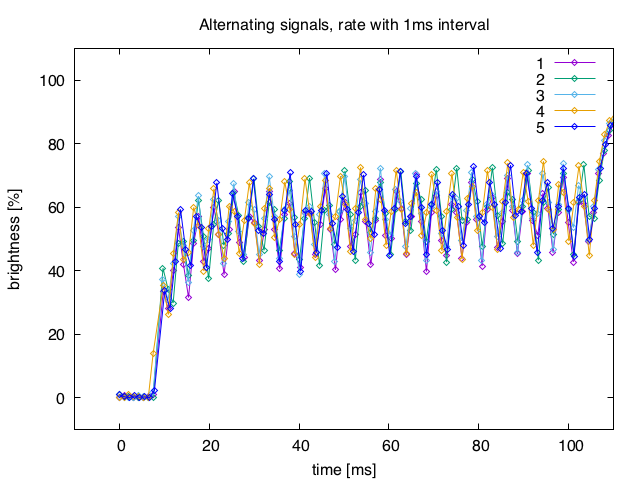
\includegraphics[height=140px]{img/overlap1}
  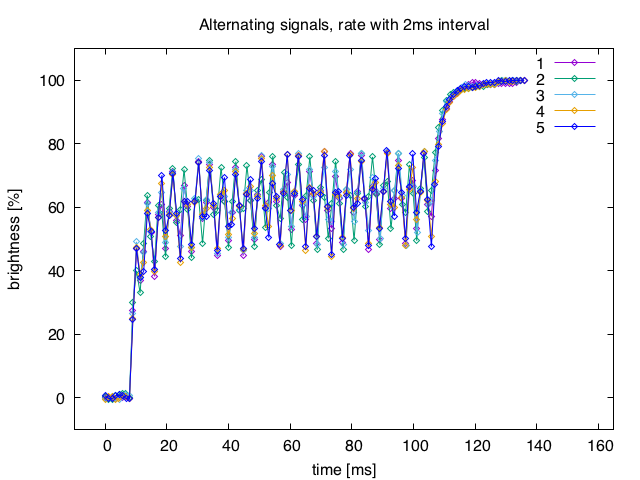
\includegraphics[height=140px]{img/overlap2}
  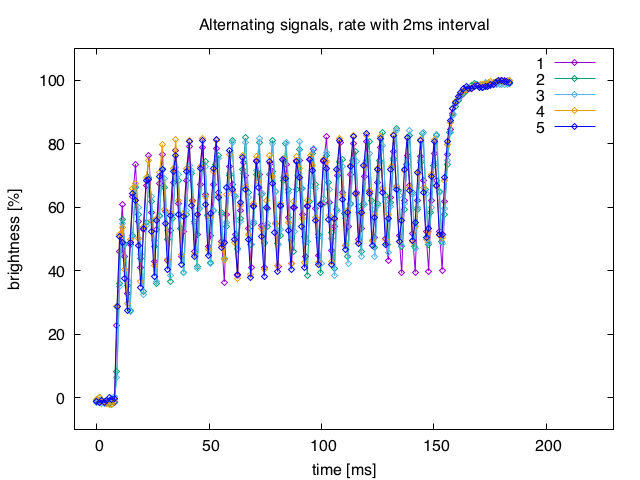
\includegraphics[height=140px]{img/overlap3}
  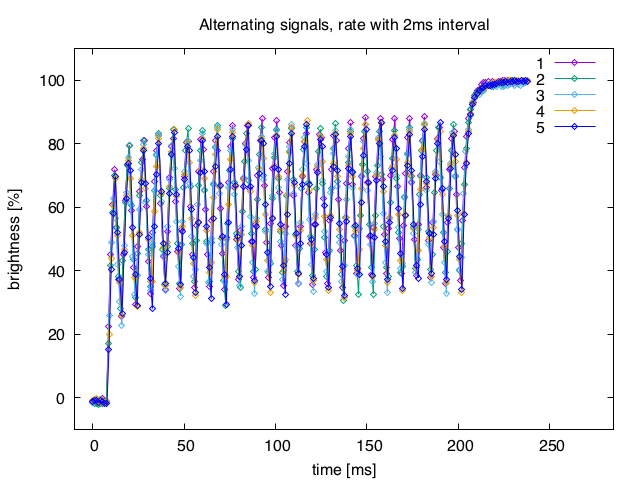
\includegraphics[height=140px]{img/overlap4}
  \caption{Test of rate with 1 ms, 2 ms, 3 ms and 4 ms intervals (left to right, top to bottom).}
  \label{fig:txpeak}
\end{figure}

\begin{table}[hbt]
\centering
 \begin{tabular}{l c c c r}
   rate interval & missing 1s & missing 0s & average 1 brightness & average 0 brightness \\
   \hline
   1 ms & 34.52\% & 30.62\% & 66.75\% +- 6.10 & 55.78\% +- 6.72 \\
   2 ms & 0.00\% & 0.00\% & 70.22\% +- 7.06 & 50.18\% +- 5.79 \\
   3 ms & 0.00\% & 0.00\% & 76.72\% +- 6.18 & 43.03\% +- 5.20 \\
   4 ms & 0.00\% & 0.00\% & 82.77\% +- 4.00 & 35.54\% +- 3.60 \\
   \hline
	\end{tabular}
  \caption{Rates results compared.}
  \label{ratestable}
\end{table}

\begin{figure}
\centering
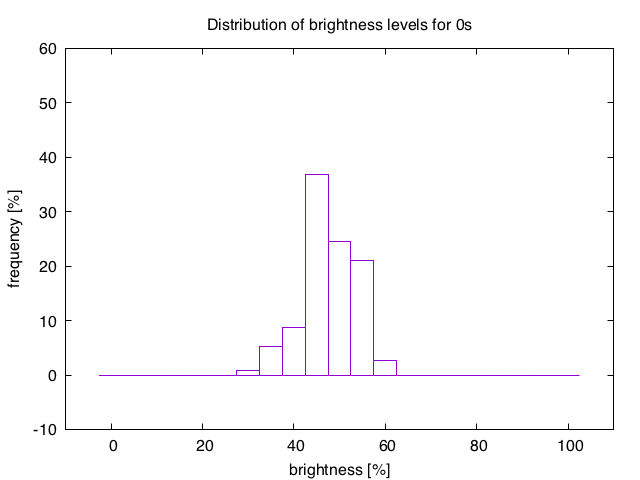
\includegraphics[height=100px]{img/hist0}
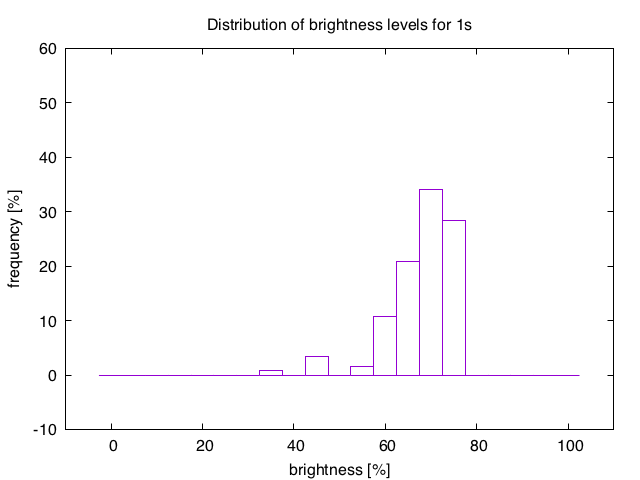
\includegraphics[height=100px]{img/hist1}
\caption{Distributions of brightness levels during transmission (2 ms interval), brightness of binary 0s to the left, 1s to the right. }
\label{fig:histopeaks}
\end{figure}


%distance
\subsection{Distance}
As we can see from table \ref{ratestable}, 2 ms is the fastest reliable rate, but how does it scale over different distances?\\
In section \ref{distancephy} it was discussed how distance influences the reception in terms of maximum brightness registered from the sensor.
However, a new relevant question is how distance would influence reception when there is transmission.
Like in the previous paragraph, an answer to this question can be found experimentally by repeatedly switching the light on and off, and measuring the characteristics of the signal that is received, at different distances.
\begin{table}[hbt]
\centering
  \begin{tabular}{l c c c c c}
    distance & max. brightness & missing 1s & missing 0s & average 1 brightness & average 0 brigthness\\
    \hline
    0cm & 100\% & 0.00\% & 0.00\%  & 70.22\% +- 7.06 & 50.18\% +- 5.79 \\
    10cm & 42.81\% & 0.00\% & 0.00\%  & 60.30\% +- 10.64 & 43.61\% +- 10.67 \\
    20cm & 14.28\% & 4.68\% & 4.68\%  & 49.99\% +- 12.22 & 36.41\% +- 12.01 \\
    30cm & 8.57\% & 2.38\% & 1.78\%  &  54.49\% +- 18.83 & 39.69\% +- 20.37 \\
  \end{tabular}
  \caption{Test of 2ms rate over different distances.}
  \label{tab:2msdistances}
\end{table}

Table \ref{tab:2msdistances} shows the results of these experiments.
Contrarily to section \ref{distancephy}, the percentages of brightness are relative to each separate experiment, in the sense that each experiment has a different level for 100\% of brightness received, depending on the distance.
For each experiment, a 100\% represents the maximum brightness measured in that experiment.
This is to shift the focus on the variations and the relation between high signals and low signals, to ultimately verify if even at different overall brightness levels transmission is still comparable.
Maximum brightness levels are still reported on the table however.
Two important aspects emerge from these results: one, that reliability remains reasonably high, and two that uncertainty in the average brightness for 1s and 0s grows a lot, probably due to the increasing weight of noise.

% big light
\subsection{Controlling AC powered lights}
As was mentioned, the control layer is supposed to control the switching of the light bulb by directly control its power supply.
This is easily achieved in the prototype since the LED is powered directly from the controller board.
However, in the optic of using light bulbs powered from AC mains, the controller layer would need to act differently.
Different switching mechanisms have been tried, and by far the most performant resulted to be a Solid State Relay switcher, or SSR for short.
A SSR has the power to close or open the circuit connected to the AC source. With a small activation signal it can allow the current to flow through or stop it.
The activation signal can easily be sent from the controller board.
Figure \ref{fig:ssrwiring} shows the wiring between the solid state relay and the Arduino board.
However, the use of a SSR brings additional limitations to the system, especially on possible speed achievable in transmission.
Although faster than other types of relays, SSRs still have some limitations, especially in the activation speed. 
Fast switching at a rate faster than the activation time of the relay will have no effect, and switching at a rate that is only slightly slower will allow only a limited amount of current through before switching off.
As the experiments suggest, the results of which shown in fig. \ref{fig:ssrwarmup}, the solid state relay is not able to convey enough current to the light bulb in less than 9 ms.
As a result, the light bulb remains switched off.
Even though the maximum brightness achieved is several times more than with the low power LED, the rate at which the LED can be controlled and modulated poses a serious limitation on the potential transmission.
In addition to this, the LED bulb has a cool down period that is far longer than the one with the low power LED, and the system would still need to implement some rectification on the current to avoid the fluctuations due to the phases of alternating current.
For all these reasons, the preferred prototype setup to achieve communication will be exclusively the one with the low power LED and direct control from the board.
Although more localised, the setup obtains higher rates of transmission, is potentially embeddable as a transceiver on a small robotic agent connected to a battery, and can achieve local communication that can be exploited in some common mobile robotics scenarios.
On the other hand, the LED bulb would have worked exclusively as an environmental transmitter, to communicate to robots externally.

\begin{figure}[hbt]
\centering
  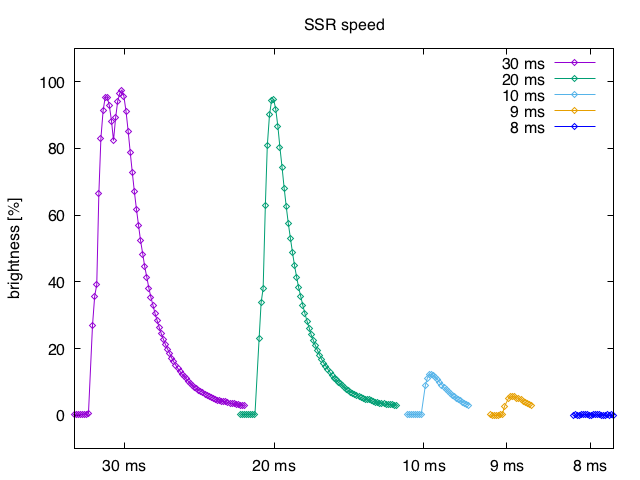
\includegraphics[height=180px]{img/ssr}
  \caption{Speed of solid state relay and light bulb setup.}
  \label{fig:ssrwarmup}
\end{figure}

\begin{figure}[hbt]
\centering
  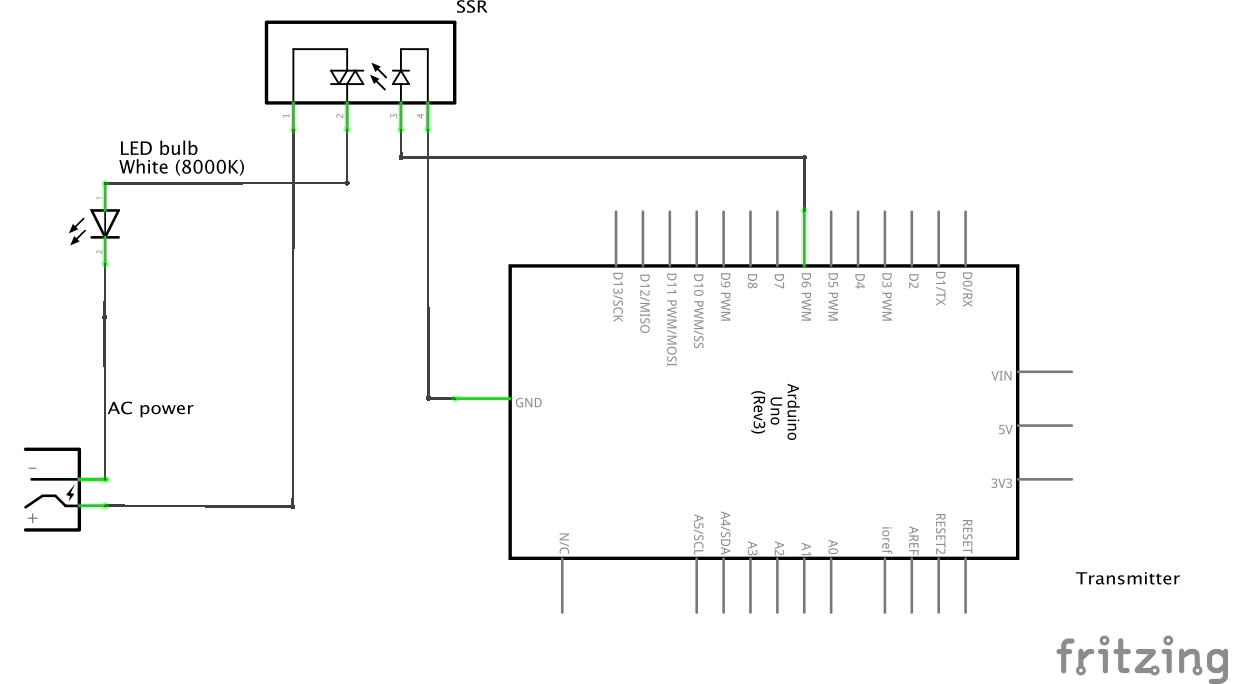
\includegraphics[height=150px]{img/ssr_schem}
  \caption{Wiring of the Arduino board with a solid state relay to control AC powered LED.}
  \label{fig:ssrwiring}
\end{figure}



\section{Logical layer}
\label{logical}
This layer represents the outermost level of abstraction, where information is handled and manipulated at a software level.
For a transmitter, the processes included in this layer regard the input of the message from a user, its encoding and communication to the control layer.
Most importantly, for a receiver module the logical layer handles the interpretation of data from the sensor back into an encoded message with meaning, its decoding and finally the presentation of the information to its final consumer.
Additionally, the logical layer is responsible of improving the reliability of the system where possible, with control mechanisms that add robustness to the unreliable aspects of the communication.
A good logical layer could handle recovery techniques in cases where symbols are missing or mistaken, and overall reduction of noise impact. 
For instance the implementation of a basic communication protocol could help in making the communication more stable and structured, allowing elementary operations such as checking correctness and encapsulation.
The complexity of the transmitter logical layer is not particularly high, the layer takes some message as input, manipulates it to meet the encoding and protocol requirements and redirects it to the control layer. 
The focus of this section will therefore be shifted to the receiving side of the communication.
The requirements that the logical layer is expected to meet are that the communication rate is not significantly slowed down by the software processes, and that communication is successfully achieved.
This final objective particularly relies on the signal recognition on the reception side.
 
\begin{figure}[htbp]
   \centering
   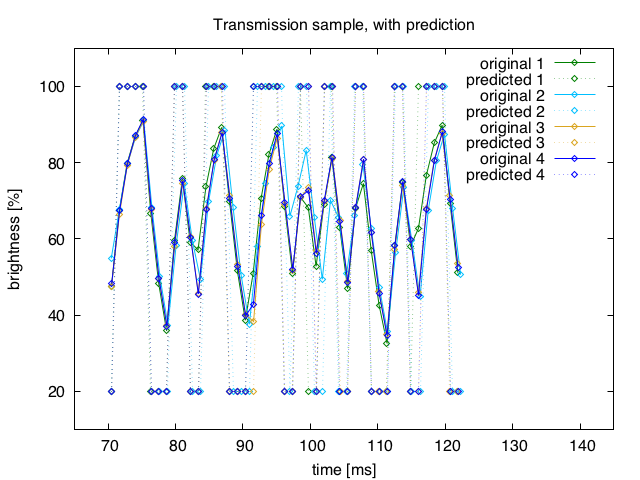
\includegraphics[height=200px]{img/sample} 
   \caption{Example of the results of interpreting digital information from analog input.}
   \label{fig:sample}
\end{figure}

%reading 
 \subsection{Reading the signal}
A key part of this layer is to convert analog sensor data representing light variations into binary code.
Fig. \ref{fig:sample} shows a sample of transmission.
The full lines, predominantly blue in the central part of the figure, represent the values registered by the sensor, while the dotted lines at the top and bottom represent a reconstruction of the digital signal.
When the analog signal comes as a sequence of increasing values, the digital prediction of the signal is  a 1, and when the sequence of values is decreasing, the prediction is set to 0.
%The green line represents the original values from the light sensor, while the purple line is a reconstruction of what the digital transmission would look like. 
Manchester encoding allows transmission to only have two kinds of peak, either representing single symbols, like a 1 or a 0, or two symbols of the same kind, like a 11 or a 00.
This is because each binary 1 is represented as the sequence 01, and each 0 as 10.
Whenever two subsequent bits are different, there will be a sequence of two symbols of the same kind in Manchester encoding.
As an example, the sequence 0 0 0 0 0 0 1 0, representing the byte 0x02, would be encoded as 10 10 10 10 10 10 01 10.
When there is the switch between a binary 0 and ta binary 1, a sequence of two 0 symbols appear in the Manchester encoded byte.
During transmission this would graphically translate to a longer and deeper 0 symbol in the reception.
The same discussion applies in reverse for a double 1.
Luckily, longer same symbol sequences are not possible with this encoding.\\
The design of an algorithm that could go through these sequences of sensory values and interpret them into binary data has undergone through different stages and different attempts.

\subsubsection{Machine Learning approach}
The first version of an algorithm for prediction made use of Machine Learning techniques to predict digital symbols given sequences of sensor data.
These techniques include the training of a model with training data, that would "teach" a classifier what kinds of sequences produce given results.
 The training data was taken in different circumstances of ambient light interference, with different messages sent and at different times.
Multiple classifiers were tested, with a maximum success rate of about 75\% of correct predictions. 
The classifiers included NaiveBayes, RandomForest, AdaBoost and ArtificialNeuralNetworks, all with comparable results.\\
There were major difficulties with this approach. 
To begin with, there were problems identifying the labels to train these models with, namely the classes or categories where the data would belong.
Initially, the four categories were "1", "0", "11", and "00". The basic idea is that given a sequence of values, its corresponding digital symbol should fall in one of these four classes.
A problem in implementing this approach was that single symbols and double symbols have sequences of values from the sensor of different sizes. 
These sizes are also called the number of features for a machine learning sample.\\
The standard module for machine learning that was used requires the same number of features for all the labels.\\
Given this restriction, the labels became "10", "01", "11", and "00". Eventually, also these labels were produced by different numbers of features, at times. Other combinations were tried, and eventually all leading to the same result. 
One way to get around this problem is to have a fixed number of features, but big enough to include all the possibilities. 
Samples smaller than this maximum amount (eventually all of the samples) would be filled up with blank values until they reach the intended size.\\
Another way would be to train a classifier for each specific number of features that may occur. In this case, the amount of classifiers needed would have been around 4, for number of features ranging between 7 and 10 with a transmission rate of 500 Hz.
The downside of this approach is that each classifier becomes very specific to a restricted set of the training data, potentially loosing track completely of certain labels.\\
The final setup for machine learning prediction used the labels "101", "100", "011", "110", "001", "11", "00", "10", "01", scaling of the features and larger sample size to be filled up with blanks.
This produced overall the best results for the machine learning approach, but never above 80\% success rate.\\
A downside to this final approach would be that when receiving values from the sensor in real time, a moving window  of the fixed size of the number of features would be necessary, and an attempt of prediction should be made at every new value inserted.
This might likely slow down the reading process.
Otherwise, it would also be necessary to keep track of the variations to only attempt a prediction when there is a switch in direction and the sequence is within a desired length.
These additional control techniques would minimise the purpose of machine learning altogether, suggesting that only keeping track of the values could be sufficient to produce a prediction.

\subsubsection{Custom algorithm approach}
These poor results ultimately led to a change of approach for reading the data, guided by the continuous adjustments performed on the previous approach. 
Just looking at fig. \ref{fig:sample} it is immediately evident that the high peaks represent 1s and the low peaks represent 0s. 
By setting some rules, a custom classifier could predict a result for a sequence of values without even the need to be trained with sample data.
In particular, the classifier analyses sequences of values, trying to find sequences that are either monotonically increasing or monotonically decreasing.
Also a noise factor has to be taken into account, in this way small enough variations are not considered.
As mentioned before, there are only two kinds of peaks in the sequences, either single or double peaks, due to the encoding of the signal.
Therefore, it is of critical importance to be able to distinguish the two cases. One criteria that was originally deployed for this was to count the number of values that progress in the same direction, either up or down. 
This was later changed to the more precise criteria of duration of such sequences, and for this reason for each sensor value a timestamp is also included in the control layer, representing the time of reception for that specific value.\\ 
With this in mind, the algorithm has been developed to very simply count the duration of either monotonically increasing or decreasing sequences of values, and produce a prediction when the direction changes, based on such duration.
This technique performs particularly well in this application, producing up to 100\% success rate in optimal conditions.
 Runtime wise, the algorithm takes constant time for each value that is received, and may or may not produce a resulting prediction.
A simplified version of the algorithm can be found in fig. \ref{code}, written in Python 2.7.\\
One aspect that is of crucial importance is the parameter called \_$doubletime$ in the code.
This parameter represents the level above which the duration of a signal is considered a double symbol.
With a continuous reception and optimal conditions, this value would be exactly the interval of time that two subsequent symbols last in the transmitter.
For a transmission rate of 500 Hz, with intervals of 2 ms between two signals, two subsequent symbols would last exactly 4 ms.
However, setting the parameter to be 4 ms would produce wrong results in many cases, due to the reception rate.
A reception rate of 1200 Hz produces a reading every approximately 0.833 ms, which means that a 4 ms interval would fall between four received values after 3.332 ms, and five received values after 4.165 ms.
In many cases, the fifth value received after 4.165 ms from the start of the sequence is already the first step to the opposite direction, therefore the sequence lasts 1 sample value less.
This is why the parameter \_$doubletime$ needs to be adjusted according to the reception rate and not the transmission rate, in this example at 3.332 ms instead of 4 ms.

\subsection{Protocol}
As can be seen the rates of transmission and reception in this prototype system are not very high, if compared to average wireless transmission speeds, which are measured in Mbps.
Transmission in visible light is also exposed to a high degree of uncertainty, depending on parameters like distance, maximum brightness, interference, noise, and so on.
In this prototype, communication is only established in one direction, which additionally increases the threat of getting wrong results.
In order to compensate all these aspects, an effort to strengthen the success rate has been made by structuring the communication into a very basic protocol.
Each message is therefore encapsulated into a Protocol Data Unit, or PDU.
Each PDU is enclosed between two single bytes: a byte STX, that indicates the start of a message, and a byte ETX which indicates its end. 
These two are bytes 0x02 and 0x03 respectively.
To avoid that the receiver wrongfully interprets an ETX byte while reading the message, perhaps as a combination of the final part of one byte and the start of another, a length byte LEN is also included in the header of the PDU, to specify the length of the message in bytes.
Additionally, each PDU is restrained to have a maximum size, and longer messages need to be split into more PDUs.
This is mostly to preserve the serial connection between logical layer and control layer, to avoid overflow of the serial buffer.
This three fields combined should make it adequately easy for the receiver to know if some parts of the message were lost during transmission.
Since the communication is established mono-directionally, the transmitter wouldn't know if the message was delivered, but the receiver most likely would.
Mistaken symbols are very unlikely in this kind of communication, it is much more likely to entirely miss some.
Therefore the receiver could easily know if the message was delivered or not, by comparing the length of the message that was initially declared and the length of the message that was received.
To increase the chances of a successful delivery, the transmitter could be transmitting the same message over and over in a mono-directional scenario.

\subsubsection{Additional fields}
Increasing the functionalities or complexity of the system, additional parameters in the PDU might result useful if not necessary. 
Imagining a scenario with multiple receivers of messages broadcasted through light in a unilateral way, a receiver ID field could be added to the PDU.
 Also, it would be wise to perform encryption on the PDUs, in a way that only the intended receivers would be able to read the message directed to them.
Establishing 2-way communication would also require more steps.
In a 2-way communication it would be much easier to ensure correctness of the transmission. 
For this, at least 2 more parameters seem necessary: a sequence number to identify the packet, and a checksum to check correctness of the received message.
When the message received is of a different length than declared or produces a different checksum, the receiving side of the communication could just ask  for the same message again, or confirm correct reception otherwise.
A header for visible light communication doesn't require many parameters in the case where a system establishes only local communication.
Otherwise for messages to travel through a network, a PDU header would also need routing parameters for origin and destination of the message.

\begin{figure}
\centering
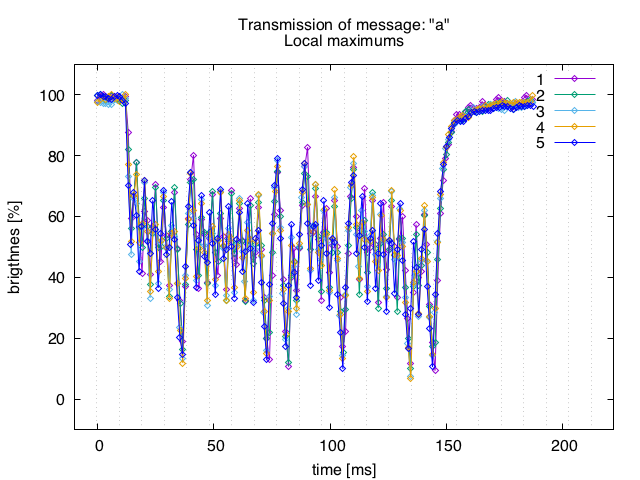
\includegraphics[height=180px]{img/transmission}
\caption{Example of transmission of message "a", the transmission include STX, ETX, and LEN bytes, over 5 samples.}
\label{fig:transmissionA}
\end{figure}

\subsection{Result}
Figure \ref{fig:transmissionA} shows an example of the transmission of the message "a", including STX, ETX and LEN bytes.
In the figure it can be seen that the transmission starts from 100\% of brightness, and returns to 100\% when it is finished. 
This is the normal operation of the communication system.
With this approach, although the rate of transmission is still fast enough to not be perceived by human eye, the perception of the light intensity drops to about 60\% during communication, as an average of high and low peaks.
This makes it possible to actually guess when there is transmission just by observing the light.
A different approach could be to keep alternating 1s and 0s even when there is no message to send, or to reduce the light intensity to a similar level during non-transmission.\\
Other than knowing when there is transmission just by observing the light intensity, it is impossible to decode the message without recurring to machines.
Once the signal as it is received is displayed graphically however, the traits of the signal in the figure can be visually associated with the Manchester encoding of the message, clearly visible at least in the occurrence of double symbols. \\
In ASCII, letter "a" is represented by the byte 0x61, or 01100001 in binary and 97 as decimal.
As previously mentioned, the STX is byte 0x02, ETX byte 0x03, and LEN in this case would be 1.
In binary, the entire message would then be: 00000010 - 00000001 - 01100001 - 00000011, as STX-LEN-"a"-ETX.\\
In Manchester encoding: 10101010101\textbf{0011}0 - 1010101010101\textbf{001 - 100}10\textbf{11}010101\textbf{001 - 1}0101010101\textbf{00}101.
A 00 and a 11 are clearly visible at the end of the first byte in the figure, at about 40 ms after the start of the sample.
 A 00 almost concludes the second byte at around 70 ms in the figure, follows a 11 connecting the second to the third byte, then a 00, 11, and so on.
 This feature of the communication also allows manual debugging during the development process.
  \todo{protocol vs no protocol?}

\subsubsection{Experimental evaluation}
To test performance of the communication in its final stage, multiple tests have been performed on the prototype.
For each test, the system takes user input for initialising the message to send, encodes it and sends it through light. 
The receiver reconstructs the message depending on values retrieved from the sensor.
Tests have been performed at very close proximity of the sensor to the light source, without other lights directly facing the sensor but with presence of natural light.
A test is considered successful if every bit is correctly received and interpreted.
Messages of different sizes have been tested.
Table \ref{tab:txresults} illustrates the results of these tests.
The message length reported on the table is measured in characters of the payload, each character represented by one byte and 16 symbols in Manchester encoding.
For each message the 3 control bytes STX, LEN, ETX are also sent and need to be added for the total length of the message.
%
\begin{table}[hbt]
\centering
  \begin{tabular}{l c c c c c}
    distance & message length (chars) & symbols in pdu &  ambient light & tests & successful \\
    \hline
   0 cm & 5 & 128 & yes & 50 & 100\% \\
   0 cm & 10 & 208 & yes & 50 & 100\% \\
   0 cm & 20 & 368 & yes & 50 & 100\% \\
   0 cm & 30 & 528 & yes & 50 & 100\% \\
   10 cm & 5 & 128 & yes & 50 & 92\% \\
   10 cm & 10 & 208 & yes & 50 & 96\% \\
   10 cm & 20 & 368 & yes & 50 & 88\% \\
   10 cm & 30 & 528 & yes & 50 & 60\% \\
  \end{tabular}
  \caption{Tests of full transmission, success criteria is 100\% correctness.}
  \label{tab:txresults}
\end{table}
%
From to these results, it is possible to calculate the probability of receiving a symbol successfully at a distance of 10 cm.
Assuming the event of receiving a symbol correctly is independent from the reception of previous symbols, the probability of receiving $x$ symbols correctly becomes $P(x) = P(1)^x$, where $P(1)$ represents the probability of receiving one symbol correctly. 
Given $P(x)$ as the probability reported on the table, this makes the probability of receiving a single symbol correctly $P(1) = \sqrt[x]{P(x)}$.
According to the results, this value ranges between $0.99903..$ and $0.99980..$ .
These results also confirm that shorter messages have a greater probability of being interpreted correctly, which makes the enforcement of the maximum PDU length rule even more important.

\begin{figure}
\centering
\begin{lstlisting}[language=Python, frame={}]
	def feed(self, time, value):
		pred = None
		
		# staying
		if abs(value - self.prev) <= self.epsilon:
			pass

		#going down
		elif value <= self.prev: 
			if self.direction: # up	
				pred = self._predict(time)

		# going up
		elif value > self.prev: 
			if not self.direction: # down
				pred = self._predict(time)

		self.prev = value
		return pred
		
	def _predict(self, time):
		m = self.direction
		delta = time - self.seqstart
		pred = '-'
		
		if delta >= self._doubletime:
			pred = '11' if m else '00'
		else:
			pred = '1' if m else '0'

		self.direction = not self.direction
		self.seqstart = time
		return pred
\end{lstlisting}
\caption{Simplified algorithm for signal interpretation (Python 2.7).}
\label{code}
\end{figure}



\section{Evaluation and Results}
%[How did it go as an application to robotics? does it make sense? performance? tests? comparisons to other communication forms?]
After all the due measurements and evaluations of the prototype from purely a communication point of view, the system was tested in the context of mobile robotics.
To evaluate the system in regards to its intended applicative scenario, a small mobile robot was equipped with a receiver module from the prototype and a Raspberry Pi to receive the information, implement the logical layer of the receiver and control the robot movements according to the messages.
 Different experiments were conducted to test the functionalities of the communication as a generic communication system with the new setup and to exploit the property of the light as a situated medium of communication.
 From the communication tests performed and presented in the previous sections, communication with a robotic agent is expected to be successful in proximity to the light source, with an adequate alignment between receiver and transmitter.

%setup
\subsection{Experimental setup}
For this evaluation the receiver has been mounted on top of a Thymio-II \cite{thymio}, a small educational robot developed  by MOBOTS, a group of the Swiss Federal Institute of Technology in Lausanne (EPFL), in collaboration with the Lausanne Arts School (ECAL).
The receiver's sensor has been placed to face in the same direction that the front of the robot faces.
The receiver board has been connected to a Raspberry Pi \cite{raspberrypi}, also mounted on top of the robot.
The Raspberry Pi provides enough computational power to implement the logical layer of the system (section \ref{logical}), and it also offers the full capabilities of controlling the Thymio robot.
Raspberry Pi and Thymio have been connected through a serial connection with a USB cable.
For the transmitter the same previous setup has been kept, with an Arduino board controlling a low power super bright LED, receiving input from a computer that takes user input.

%components
\subsubsection{List of components}
\begin{enumerate}
\item Photoconductive Cell VT900
\item Genuino Yun micro controller board, based on ATmega32u4 \cite{arduinoyun}
\item Raspberry Pi 3 Model B to be applied on a mobile robot
\item Thymio-II educational robot
\end{enumerate}

\subsubsection{Wiring}
Figure \ref{fig:wiring2} shows a diagram of the experimental setup.

\begin{figure}[hbt]
\centering
  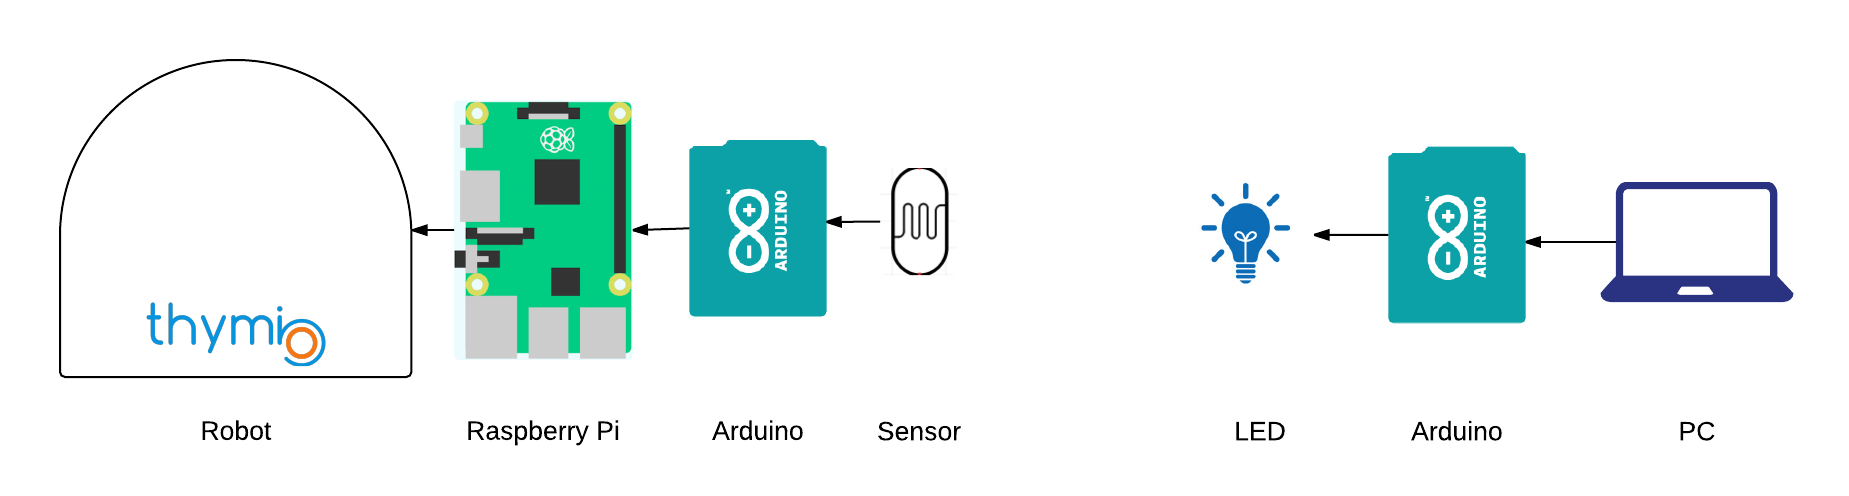
\includegraphics[width=400px]{img/wiring2}
  \caption{Experimental setup.}
  \label{fig:wiring2}
\end{figure}

%experiments
\subsection{Experiments}
The \textbf{first experiment} that has been performed was to test the overall capabilities of the communication system with the new setup.
The experiments merely consisted of transmitting movement instructions like any common remote control.
The commands tested were: forward, backwards, left, right and stop.
Commands were taken from user input on the computer controlling the transmitter, and transmitted through light.
Upon reception, the receiver would then control the robot's movements accordingly.
\newline
A \textbf{second experiment} was conducted to exploit the property of this communication system of being situated and simultaneously its potential to virtually send any message, not only preprogrammed commands.
In this experiment, two more photoresistors were connected to the receiver module, and their values forwarded to the logical layer alongside the one used for reading the signal.
The three sensors are all placed facing forward in regards to the robot's direction, with the central one facing forward and the two on the sides in diagonal to get a view of the sides.
Figure \ref{fig:thymioangles} shows the placement of the sensors graphically.
%
\begin{figure}[hbt]
\centering
  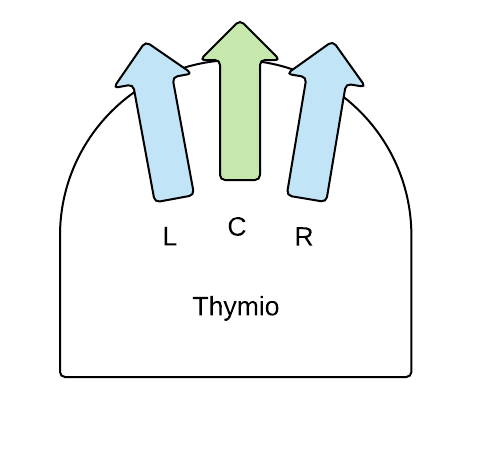
\includegraphics[height=100px]{img/thymioangles}
  \caption{Placement of the sensors in front of the robot.}
  \label{fig:thymioangles}
\end{figure}
%
The central sensor is the only one from which the values are read for communication, while all three help in the determination of the light source's direction in relation to the robot.†
The robot is programmed to always face the light source, and turn to the side which sensor registers more light, above a certain limit.
The experiment consists of reprogramming the robot's behaviour based on the message sent encoded in light.
When the message instructs to approach the light source, the robot actively follows the light source moving forward.
When the message instructs to move away from the light source, the robot moves backwards away from the light source, still facing its direction.
This is an example of messages that potentially reprogram the behaviour of the agent, adding as a plus information about relative position of the source of the message.
To distinguish this case from a case of preprogrammed reactions to specified commands, the message contains the velocity parameter that the robot needs to apply to its motors, instead of merely say 'forward' and 'backwards' like in the previous experiment.
When the velocity is positive, the robot approaches the light source, following it and moving forward, when the velocity is negative the robot will evade the light source moving backwards away from it.
Depending on the specific value contained in the message, the robot will move at different speeds.

This experiment is intended to demonstrate that a communication system that allows generic communication can be used to transmit a wide range of complex instructions, represented in this experiment as a wide range of potential values for the same parameter, velocity in this case.
The fact that the system exploits a form of situated communication adds to the message the information of direction and positioning relative to the source of the message.
Rather than programming a robot to present a behaviour in reaction to a predetermined command, the experiment directly instructs the robot to exhibit the new behaviour, represented by a velocity of adaptable intensity and direction.
Therefore, the behaviour is not known to the robot beforehand, but is dynamically received and executed.
Encoding predetermined commands into finite sets of signals could result limiting in certain applications, while instead this way of communicating instructions can arguably produce an infinite range of possible outcomes.
Dynamic instructions could prove decisive in applications where behaviours need to be adjusted depending on variable circumstances, or where the set of instructions is just too large to be mapped to distinct signals within a reasonable effort.
%
%The same effect could be achieved by a system that uses two separate communication subsystems, one reactive and situated, like a coloured light or an infrared sensor, and another generic and local, like could be Bluetooth.
%If two agents have the ability to identify each other, generic communication could be exchanged through another wireless channel.
%This technique however would present considerable issues in the case where multiple agents 
%A visible light communication approach however would reduce complexity and achieve the same result, provided that the performance is considered sufficient.

When running the experiments initially, the transmission rate adopted was the one with 2 ms intervals between each symbol.
This led to poor results and bad reception over distances greater than 10 cm, and was later changed.
The final transmission rate that was chosen was half the previous, at 250 Hz with 4 ms duration of each symbol.

%results
\subsection{Performance and Results}

The two experiments were evaluated separately in terms of quality of reception and success rate.
Factors that influence the outcome of the experiments are also taken into account, like distance, angle and interference.

\subsubsection{Remote control}
For this experiments, the system has been tested and evaluated as a generic communication  medium to perform remote control of the robot.
A restricted set of commands is known to the receiver, that has been preprogrammed to react to each of them in a distinct way.
The commands represent movement instructions.
Table \ref{tab:remotectrl} shows the results of these experiments in the best experimental conditions and with a transmission rate of 250 Hz (4 ms intervals).
\begin{table}[hbt]
\centering
  \begin{tabular}{l c c c c}
    distance & angle & interference & tests & success rate \\
    \hline
   0-10 cm & direct ($< 15^{\circ}$) & low & 50 &  50\%\\
   10-20 cm & direct ($< 15^{\circ}$) & low & 50 & 20\%\\
   20-30 cm & direct ($< 15^{\circ}$) & low & 50 & $5\%$\\
  \end{tabular}
  \caption{Results of the remote control experiment.}
  \label{tab:remotectrl}
\end{table}
Experimentally, the system appears very sensitive to the exposure to the light source, in terms of angle and facing direction.
The LED used for these experiments has a limited viewing angle of nominally $30^{\circ}$, but the sensor needs to face the centre of the light source to receive the signal correctly.
Facing other directions will greatly reduce the chances of success, even with low deviations.

An effort to slightly increase the success rate with selected commands can be done by comparing a received signal to the possible known outcomes, when the signal is incomplete or wrong.
By computing the edit distance between what has been received and each of the expected commands, the known command more similar to the received message is also the most likely.
This technique could improve the success rate at the cost of a higher computational burden.
An ideal condition to optimise it's effectiveness is the use of possibly short commands from a restricted set, and fairly distinct to one another.

\subsubsection{Situated dynamic behaviour experiment}
This experiment is composed of three different stages: the development and testing of two separate parts, and the final experiment with the two merged together.

First, the reception process need to be adjusted to take values from multiple light sensors instead of just one, and to control the robot so that it always faces the direction with the higher brightness intensity at any time.
Second, specific instructions need to be sent as messages, so that the robot doesn't have any knowledge of commands or behaviours beforehand, but executes the commands as they come in form of messages.
Finally, combining the two parts, the robot will have one behaviour preprogrammed, that is to face the light source, and one dynamically set through the message sent to it, that is how to act in relation to the light source.

The first part might represent a bigger challenge than it might seem.
Taking analog input from one source can be a computationally demanding process since it can slow down the clock rate significantly due to the analog-to-digital conversion process.
Reading analog input from three different sources though is expected to be exactly three times slower than reading only from one source.
The accuracy of the new transmission rate is therefore scaled with the lower reception rate.
With a reception rate of 1200 Hz, a transmission rate of 250 Hz (4 ms intervals) is highly accurate in close proximity, and more robust to distance than faster rates.
With three sensors however, the reception rate drops to 400 Hz, three times slower than before.
This new reception rate brings down the accuracy of transmission.
Where before the transmission of a single symbol could be registered as a sequence of about 5 values from the sensor (1200 values per second means 1.2 values per millisecond, which results in 4.8 values for 4 ms), with the new rate each symbol is only about 2 values long.
This brings the precision of the new setup between the ones from the 1000 Hz and 500 Hz rates of the previous setup with only one sensor.
Therefore, it's plausible to expect a drastic drop in accuracy with this setup.

The second part of the experiment has virtually no real difference with the first experiment, since the system allows the exchange of generic binary data that can represent virtually anything.
The only adjustment that needs to be made is to send parameters instead of commands, and how the receiver responds to them.
%
\newline
\begin{table}[hbt]
\centering
  \begin{tabular}{l c | c c || c c}
  distance & angle & interference & success rate & interference & success rate\\
    \hline
    0-20 cm & $90^{\circ}$ & no & 10/10 & yes & 10/10\\
    0-20 cm &  $180^{\circ}$ & no & 10/10 & yes & 10/10\\
   20-40 cm &  $90^{\circ}$ & no &10/10 & yes & 10/10\\
   20-40 cm &  $180^{\circ}$ & no &10/10 & yes & 10/10\\
   40-60 cm &  $90^{\circ}$ & no & 10/10 & yes & 10/10\\
   40-60 cm &  $180^{\circ}$ & no & 10/10 & yes & 10/10\\
   60-80 cm &  $90^{\circ}$ & no & 10/10 & yes & 10/10\\
   60-80 cm &  $180^{\circ}$ & no & 10/10 & yes & 10/10\\
  80-100 cm &  $90^{\circ}$ & no & 10/10 & yes & 8/10\\
  80-100 cm &  $180^{\circ}$ & no & 10/10 & yes & 7/10\\
  \end{tabular}
  \caption{Results for robot turning towards the light source, with and without interference.}
  \label{tab:turning}
\end{table}
%
Table \ref{tab:turning} shows the results of the behaviour of the robot to turn towards the light source.
The experiment was conducted placing the robot on the line of the light source, but facing in a different direction.
The two directions tested were perpendicular ($90^{\circ}$) and opposite ($180^{\circ}$).
The success criteria is the ability of the robot to turn until it faces the light source, stopping when perfectly aligned.
In this experiment, the robot is only allowed to rotate, but not move otherwise.
As can be seen, this first part of the experiment had a high success rate within a close range to the light source.
At longer distances however, the light becomes harder to spot, especially with interference from other sources.
In a dark environment, the presence of reflecting surfaces close to the robot can cause a reflection to be interpreted as the source of the light, where the robot can get stuck if the actual source is not in sight.
An important result of this test is that the light source can be seen from much farther away than the distance necessary for actual communication, making it potentially possible for a robot to approach the source of transmission and enhance the chances of a successful communication.

\begin{figure}[hbt]
\centering
  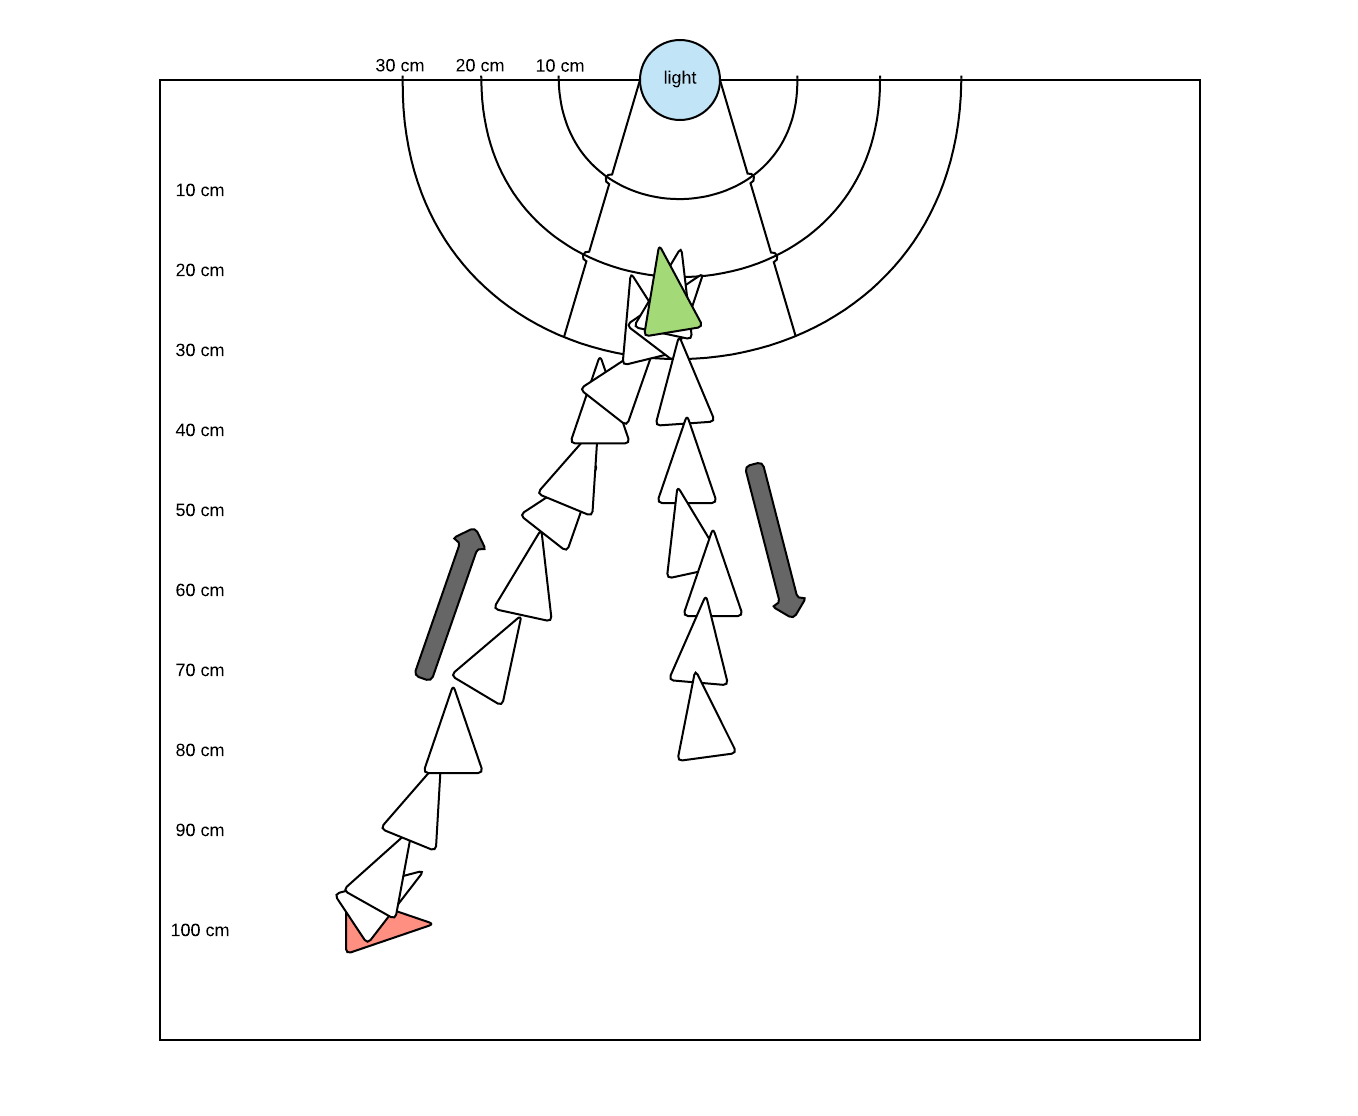
\includegraphics[height=250px]{img/experiment2}
  \caption{Graphical representation of final experiment.}
  \label{fig:experiment}
\end{figure}

This is in fact what happens in the final experiment.
Figure \ref{fig:experiment} is a graphical representation of the final experiment, based on the observation and video recording of its proceeding.
The experiment was run multiple times, the figure however only represents a single instance representative of the whole.
In the figure, the robot is represented by a triangle, and its front by the smallest angle of the triangle.
In the experiment, the robot starts at approximately $1 m$ distance to the light source, the position is represented by the red triangle.
Its initial behaviour is to follow the light source by always facing in its direction and advance.
The transmitter continuously sends the same message at fixed intervals of 1 second.
The message sent contains a negative velocity.
At the initial distance, the robot is only able to identify the direction of the source, but is not able to decipher the message.
As a result, the robot continues to advance to closer ranges.
After several attempts, when the robot reaches a distance between $20$ and $30 cm$ from the source, it is also able to correctly interpret the message.
In the figure, the position of the reception of the message is represented by a green triangle.
In this experiment, since the message sent is a negative velocity, the moment of reception is easily observable since the message causes the robot to retreat away from the light.

An unexpected behaviour that presented itself multiple times is that once the robot enters an area between $30$ and $50 cm$ from the source and is centred in regards to the source's position, it readjusts its direction more often than usual, hesitating and advancing more slowly.
Due to the narrow angle between the front sensors and the distance from the source, the three front sensors are hit by a comparable intensity of light, causing random noise to dictate one direction in favour of another, multiple times.
When this happens the robot immediately readjusts, and the same happens over and over, causing the robot to slow down its advancement.
This ultimately leads to more time spent in direct sight of the signal, which in turn causes the robot to receive the message at longer distances than expected, for the reason that advancement is slower.

\todo{angle part with multiple sources?}











\section{Discussion}
%[This is some discussion.Here I can link my results to the vision that was presented in the introduction, are the results good enough for some of those applications? Are those scenarios plausible according to my findings? what could be done with my system, more than what has been done? How could one take my work and use it for other purposes, or expand it? how to make it faster? √ ]
%why not infrared?? VL is user friendly, easily restrained, more local
After the analysis and evaluation of the prototype system, downsides and potential of visible light communication appear more defined, especially in the context of mobile robotic communication.
A do-it-yourself system implemented with general purpose hardware by no means achieves the impressive performances documented in research, however it can provide a quick to implement and easy to use form of situated communication.
Using a low power LED can achieve generic communication locally to the source, although subject to alignment and distance limitations in practical usages.

%cons
\subsection{Downsides}
The system has some clear downsides in terms of performance, but most of them depend at least partially on hardware and platform characteristics rather than on physical properties of the technology as a whole.
One major limitation is distance. The use of a low power LED only achieves a few centimetres of transmission range.
In the specific case that was evaluated, a distance of about 30 cm has been experimentally found to be approximately the maximum distance at which signals can be received correctly.
However, the direction of the light source can be seen at longer distances, making it possible for mobile devices like robotic agents to approach the light source in order to receive messages.
This limitation is mostly due to the available power, upon which depends the choice of LED to be used in the system.
The power source directly affects brightness of the LED and hence the range where it is visible.
High power LEDs are in general also brighter, and can be seen at longer distances.
Also, the brighter a light is, the less interference will play a role in reception, allowing greater ranges of communication.
Research has proven much greater distances achieved with visible light communication, from a few meters to a few kilometres \cite{ronja}.
Having access to and control of high power sources would make the communication system operate at wide ranges when necessary.

Another important limitation of the system is in the exposure of the sensor to the light source.
This factor can also depend on the light source.
The LED used had a limited viewing angle, so any sensor pointing outside of this range would not register accurate variations.
Light sources with wider viewing angles and higher intensities can be seen even without optimal alignments, and research suggests that when the light source is bright enough, good levels of exposure can be achieved with light reflection from the walls or other surfaces\cite{interferenceVLC}.
This includes not only angles in two dimensions, but in three. A sensor directly facing the light source, but pointing to positions above or below it, will be much less effective.

Finally, the speed of the communication that was achieved is very low compared to modern standard communication technologies.
Like the other limitations, this can also be a hardware dependent factor.
Faster controllers and faster switching LEDs would achieve greater speeds both in reception and in transmission.

%pros
\subsection{Advantages}
Limitations in power and distance can be also viewed positively in certain applications.
For the fact that these characteristics of the communication are influenced heavily by the hardware, light signals can be easily restrained to achieve communication types that fit the specific application. 
A choice on the hardware can restrict or expand any characteristic of the communication, including brightness and distance (type of light emitting device and power available), angle of view (type of light source), and speed (clock rates, power and speed of light source).
Depending on the application, different hardware setups could provide the optimal signal characteristic without further configuration, for example the prototype system that has been tested can only achieve local communication at relatively slow rates mostly due to the hardware setup.
Different choices on the hardware could make systems adapt to their specific application.
Whether an application requires long range communication, or local, or perfect alignment source-to-destination, or high rates of transmission, VLC systems are very flexible and can be adjusted to fit the scenario perfectly, also due to the high variety of light emitting devices that can be exploited.
Additionally, hardware is not the only factor that can influence the characteristics of the communication.
Physical boundaries can also be applied to the environment to further restrict and localise the communication, and the signal can be manipulated with the aid of simple optical techniques involving the use of lenses and mirrors, to redirect, spread or concentrate the signal.
Ultimately, physical characteristics of light such as speed, easy restrain and redirection, absence of electromagnetic interference, are the ones that made the success of fiber optic communication. 
These same characteristics can be exploited also for wireless communication using light.
\newline
Finally, light is a form of situated communication, meaning that in addition to achieving generic communication, a VLC system also allows to determine the relative location of the source of the message.
This property can be exploited in multiple applications, and is especially useful for swarm robotics for the reason that it allows both local communication and mutual localisation of the agents.

%comparison, why visible light?
\subsection{Comparing technologies}
Other forms of communication could achieve the same as visible light.
Even in the same context of swarm robotics, local, situated and generic communication can be achieved with a \textbf{hybrid system} composed of two components, one component to give direction or identify and localise a source of transmission, and a second one to actually perform the communication.
%
%The same effect could be achieved by a system that uses two separate communication subsystems, one reactive and situated, like a coloured light or an infrared sensor, and another generic and local, like could be Bluetooth.
If two agents have the ability to identify each other through the situated component, generic communication could be exchanged through another wireless channel, like Bluetooth.
This technique however would present considerable issues in the case where multiple agents are in the same communication range.
Furthermore, removing entirely the situated component from the system would still allow two agents to communicate and mutually localise each other, through the use of a shared reference system and possibly indoor positioning techniques.
A visible light communication approach would however reduce complexity and achieve the same result faster, provided that the performance is considered sufficient in the given application.

Also communication with signals in the bands right next to visible light, namely infra red and ultra violet, share similar characteristics with visible light.
Compared to those, visible light has the advantage, by definition, of being recognised by the human eye.
This characteristic allows an immediate interaction with humans, that can easily verify if the device is transmitting anything or not, or if the receiver is in line of sight with the source.
Light emitting devices are also largely available in the market and in everyday life, building a communication system on top of them will add to the light the feature of communication, and similarly the communication system will have the unique feature of providing illumination too.
 % also a lot of lights around, indoors especially, advantage or comparison?
%Why not use infrared then? it's still light. If it's visible however it's human friendly, easily restrained, safe, local.

%applications
\subsection{Applications}
VLC systems can have a wide variety of applications for their characteristics.
Local communication for mobile robotic agents has been largely discussed.
The mobility of the agents is a trait that can exploit the localisation of the source, making the robots potentially act on it.
In general, VLC systems have been already deployed as indoor positioning systems, for multiple reasons.
Lights indoors are already present in most places, and there is still an open search for the perfect indoor positioning technology, since GPS does not work indoors.
Smart spaces could also be implemented using visible light, providing localised services in specific places.
One interesting application of visible light communication would be to exploit street lamps to provide cars with information about possible directions, potentially allowing self driving cars to by guided by the street lamps already present on most roads. 

%local and situated, good for robots and local communication like swarm robotics.
%in general, good for indoor positioning, or indoor smart localised services.
%\todo{street lamps, navigation on roads}

%go faster, ADC stuff mostly
\subsection{Faster communication}
Transmission and \textbf{reception rates} with generic purpose Arduino boards are surprisingly low, for boards with clock rates of 16 MHz. 
However, multiple factors have to be taken into account.
Just focusing on the receiver, even though reading from analog input should in theory be performed as a constant amount of CPU instructions, the analog-to-digital converter (ADC) slows down the clock rate significantly to achieve a good resolution.
The ADC needs to convert an analog value from a continuous domain in continuous time to a digital value in a discrete domain and discrete time.
To do this, the ADC samples the analog values at given intervals depending on the sampling rate, and rounds them to the closest digital value they can reach depending on their precision. 
Arduino boards also use a prescaler to reduce the frequency for the ADC clock in order to obtain better resolution in the conversion.
The AVR ADC of the Arduino board has a recommended clock speed of between 50 kHz and 200 kHz when 10 bit resolution is desired, according to the producers \cite{atmel}, above this rates the resolution starts to degrade.
To achieve the lower clock speed, the original clock rate of 16 MHz needs to be scaled down by integer division with a prescale value.
Prescale values of 2, 4, 8, 16, 32, 64 and 128 are provided. 
This means that the prescale will be set to 128 for analog reads in Arduino, making the new rate 16 MHz / 128 = 125 kHz, since a prescale of 64 still produces a rate that is too fast (250 kHz).
On top of that, a normal conversion in the ADC takes 13 ADC clock cycles, still according to the producers.

The hardware limit for the sample rate of analog input will therefore become 125 kHz / 13 = 9600 Hz.
There are several ways to speed up this process though, one could be to change the core clock down to 12 MHz. 
After prescaling and performing the 13 instructions, the limitation of the sample rate would become 12 MHz / 64 / 13 = 14 kHz, because a prescale factor of 64 would be enough in this case.
Another option is to manually change the prescale factor at the expense of the accuracy level.
A prescale factor of 16 would result in a much faster rate of 1 MHz / 13 = 77 kHz, and according to the producer of the ADC, "frequencies up to 1 MHz do not reduce the ADC resolution significantly" \cite{atmel}. 
These aspects were not taken in consideration when designing the prototype, but these options could be implemented to achieve faster rates of transmission even with the same hardware.
More performant hardware is also a valid option.

%future work
\subsection{Future work}
This project only went as far as preliminary tests with robotic agents, to demonstrate a proof of concept.
A natural next step would be to test the system thoroughly in different applicative scenarios, mainly involving robotic agents but it could be a possibility to explore even entirely different contexts.
In preparation of this, several adjustments can be made to the \textbf{hardware}.
First of all, the system can be made a transceiver, able to both transmit and receive by merging the transmitter and receiver modules in a single system instead of two separate ones.
This would allow much more versatility in the potential applications where the system could serve a useful purpose.
To make the system faster and more portable, more specialised hardware can be used or designed ad hoc, rather than the general purpose platforms employed in this project.
For mobile robotics, size can be an important factor, and embedded specialised circuitry could easily make a prototype several times smaller and more efficient.
The robot utilised for the evaluation, the Thymio-II \cite{thymio}, is a full system external to the communication module, complete with a set of software tools that allow an external terminal to control it and program behaviours.
If instead the communication module were embedded into a robotic system, directly connected to the central brain of the robot itself and hence with direct access to motors and actuators, several passages of the system architecture necessary for the current prototype could be avoided entirely.
Embedding a smaller and lighter communication module into a robot could be a first step for an extensive evaluation of the system in various \textbf{scenarios}.
Examples of these could be in swarm robotics, where independent agents need to coordinate or share information.
A specific case could be when agents need to merge to form larger organisms.
In this case, agents need to be able to localise one another, approach, and perhaps communicate the way in which they need to connect or interact.
A communication system that could make these interactions simpler could use visible light or infrared signals. 
Another application of a small embedded VLC transceiver could be in multi robot exploration.
When getting close, robots could exchange information about their knowledge of the explored surroundings.
Environmental transmitters could also be developed as a continuation of the work carried on so far.
Lamps placed in one room could transmit to robots present in the room, establishing environment to robot communication.
 Perhaps robots could be provided with aid for navigation or instructions to follow in this case.

\section{Conclusion}
%[This is the conclusion.Here I sum up all the crucial points of my work, from the vision, to my results, to some of the major points in the discussion.]
\todo{how did it go with the requirements?}
%
Visible light communication is a good candidate to achieve local, situated communication.
These two properties combined make it a suitable form of communication to be used in the context of mobile robotics, to achieve robot-to-robot and environment-to-robot communication.
The development and evaluation of a prototype system using general purpose hardware and platforms demonstrate how easily communication can be achieved within certain boundaries.
The prototype can achieve local communication within 30 cm of range in direct line of sight source-to-destination.
If mounted on a robot, the system is able to identify the light source from farther distances and with different angles, although reception of messages has not been established from afar.
The mobile robot however can be programmed to approach the light source, so that when it comes in range, messages are correctly received.
The minimum rate for the communication to be successful is of about 500 Hz with the given hardware setup, but lower rates achieve higher accuracy.
Even at this low rates, errors in reception are still present, but a simple protocol allows the receiver to acknowledge when they occur.
Since only mono-directional communication has been established, the transmitter sends the same message repeatedly.

Hardware characteristics of the system can potentially help increase the performance of the communication in most measurable ways.
For this reason, VLC systems can be extremely flexible and adaptive, a choice on hardware components can influence many aspects of the communication as the application requires.
Some of the strong points of visible light communication are that light emitting devices like LEDs are generally cheap, available, human friendly and with low power consumption.
As a plus, light is not subject to electromagnetic interference, exploiting an entirely different band in the spectrum.
In the context of mobile robotics, a VLC system can achieve local communication since light is easily restrained by hardware and physical barriers, and most importantly it allows localisation of the transmission source.

In this like in other contexts, this medium of transmission can exploit a large amount of light emitting devices already present everywhere to achieve environment-to-device communication, providing additional functionalities other than illumination first among which indoor positioning.

Visible light is not the only form of communication that can achieve this, also signals in the non-visible spectrum have similar properties, like infra red and ultra violet.
Additionally, non situated forms of communication can be extended with a situated component to form a hybrid system, or adjusted with techniques that can allow the source of the communication to be identified and localised while exchanging generic information.
Visible light however can be recognised by the human eye, allowing an immediate way for humans to determine if the system is running in a correct way and to interact with it.
In some applications, a communication system using visible light could also provide illumination as an additional feature, other than just communication.


\clearpage
\bibliographystyle{plain}
\bibliography{report}
\end{document}